\documentclass{article}
\usepackage[utf8]{inputenc}
\usepackage{gensymb}
\usepackage{physics}
\usepackage{enumitem}
\usepackage{listings}
\usepackage[margin=0.5in]{geometry}
\usepackage{graphicx}
\usepackage{float}
\graphicspath{ {Images/} }
%\usepackage{amsmath}
\usepackage{amssymb}
\usepackage{qcircuit}
\newcommand\tab[1][1cm]{\hspace*{#1}}
\newcommand\coolleftbrace[2]{%
#1\left\{\vphantom{\begin{matrix} #2 \end{matrix}}\right.}
\newcommand{\tens}[1]{%
  \mathbin{\mathop{\otimes}\displaylimits_{#1}}%
}
%\usepackage[final]{pdfpages}


%\usepackage[spanish]{babel}    
\usepackage[T1]{fontenc}
\usepackage{natbib}
%\usepackage{array}
%\usepackage{gensymb}
\usepackage{indentfirst}
%\usepackage[table,xcdraw]{xcolor}



\title{Quantum Interference and Entanglement Lab}
\author{Joshua Levy\\Lab Partner: Alex Chuang}
\date{UC Berkeley Physics 111B\\April 2017}


\begin{document}

\maketitle

\section{PreLab and MidLab Sign Offs}
\begin{center}
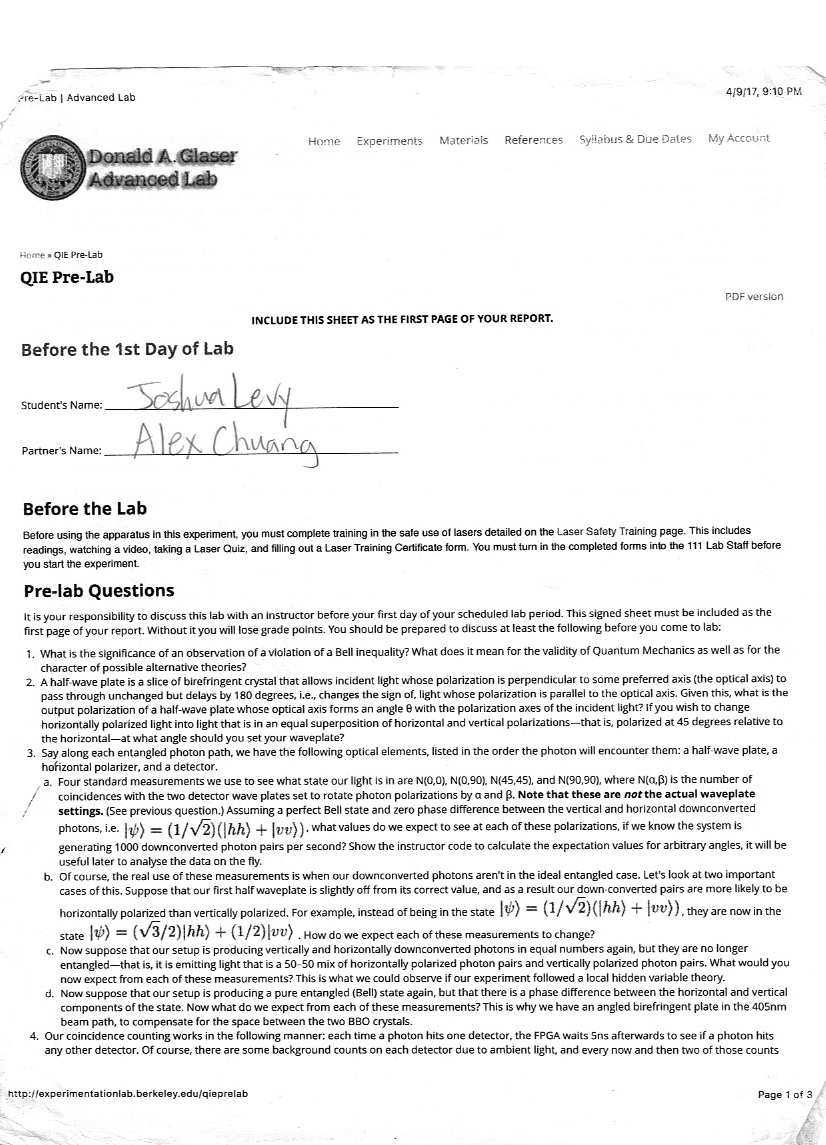
\includegraphics[scale = 0.3]{PreLab1.jpeg}
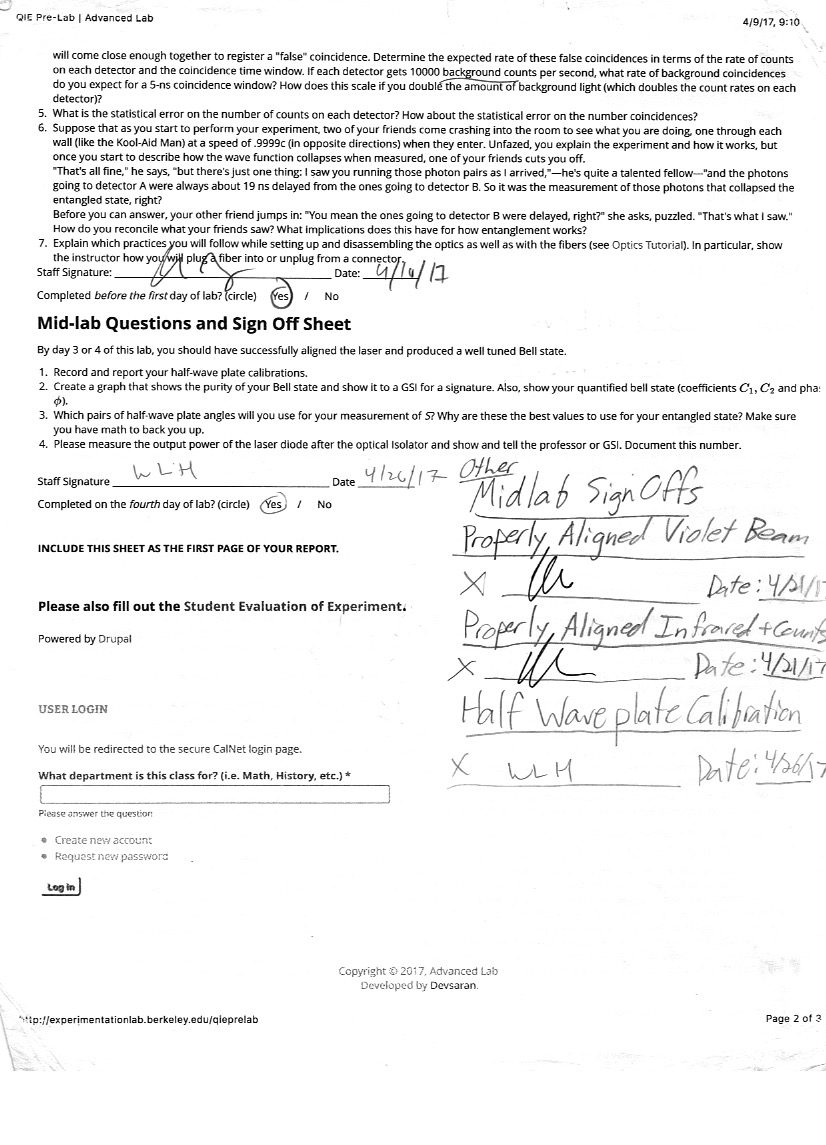
\includegraphics[scale = 0.3]{PreLab2.jpeg}
\end{center}

\newpage


\section{Abstract}
    My partner and I studied the effects of quantum entanglement of photon polarizations in order to disprove local hidden variable theories as a descriptor of nature. We rotated the polarization of horizontally polarized photons emitted from a violet laser diode and used the process of spontaneous parametric downconversion via two nonlinear crystals to generate photon pairs entangled by their polarizations. The entangled state can be tuned, so we tuned the state ($\ket{\psi} = cos\theta_l \ket{HH} + sin\theta_l e^{i\phi} \ket{VV}$) in an attempt to create a bell state, $\ket{\Phi^+} = \frac{1}{\sqrt{2}}(\ket{HH} + \ket{VV})$. We tested the purity of our bell state  by measuring $\theta_l$ (expected value of $45\degree$) and $\phi = \delta + \phi_l$ ($0\degree$ expected value), and found for our produced state, $\theta_l = 45.024\degree \pm 0.181 \degree$, and $\phi = 8.5233\degree \pm 9.108\degree$, which indicated a pure bell state. By rotating the bases of each photon's polarization in this state via half-wave plates and measuring coincidence count rates for various half-wave plate settings as outlined by Dehlinger \cite{deh}, we found strong correlations between the polarizations of the entangled photons and violated CHSH's version of Bell's inequality ($|S^{(HVT)}| \leq 2$) by measuring S to be $S_{day one} = 2.4855 \pm 0.0172$ and $S_{day two} = 2.4750 \pm 0.0179$ over two separate trials. This result contradicts local hidden variable theories as introduced by the EPR paper, and affirms quantum mechanics as an adequate descriptor of nature.


\section{Introduction}
    The theory of quantum mechanics discusses  remarkable effects occurring in the world of elementary particles. Such a theory is a great descriptor of natural phenomenon, but is quite paradoxical and at times, very unintuitive. Quantum mechanics relies on three main principles: superposition, measurement, and unitary evolution. The first principle describes how a particle can be probabilistically superimposed between multiple states simultaneously, and the second principle tells us how measurement can change the state of the particle and what we can know about its properties. The last principle discusses how the state changes over time. For the case of this experiment, we will be studying 2-state quantum systems, which we can call qubits. We can encode the information of a qubit in many different ways, which may include the use of atomic orbitals, josephson junctions, SQUID devices, photon polarization, and the spin of a particle. This experiment will utilize a photon's polarization to describe a qubit.\cite{vaz}
    
    We can combine multiple particles together to form quantum states of several particle systems. In the case of a two qubit (or multiple qubits for that matter) system, the resulting quantum state can be entangled, that is, the state of the system cannot be factored into individual quantum states. If we measure one particle, we can immediately deduce the state of the other particle under the "Copenhagen" interpretation of quantum mechanics, that the measurement of one particle immediately collapses the quantum state of both, regardless of their localities. What we know about one particle, we can know about the other through a strong correlation. The polarization of two entangled photons classically should have no correlation between the two, but in the quantum realm, we should see that the two are in fact correlated. 
    
    This notion of entanglement was disputed none other than by Albert Einstein, who noted an apparent contradiction between the uncertainty principle, which states that you cannot simultaneously know the position and momentum of a particle (the principle is applied to many other types of observables), and entanglement. For two entangled particles, he thought, what if we could measure the position of one entangled particle and the momentum of the other. Thus know the position and momentum of each measured particle's counterpart, allowing us to violate the uncertainty principle by knowing both position and momentum. How could the outcome of the second particle depend on the first when the two are noninteracting? A few years later, Einstein, Podolsky and Rosen \cite{deh} \cite{bell} published the EPR paper, a mathematical attempt to describe this paradox, and was an attempt to discredit quantum mechanics as incomplete in favor of the local hidden variables theories (HVT/LHVT), that the world is not in fact truly random and that we just have a lack of knowledge about additional degrees of freedom in a system. They posited that their are other factors interfering with the system that we do not know about, which when uncovered, would show that quantum mechanics, in its probabilistic nature, does not adequately describe nature. The EPR Paradox is not merely limited limited to the position-momentum problem.
    
    Suppose we entangle two particles and separate them at very far distance, such that the time it takes for light to travel between the two of them is not fast enough to explain the correlation between the two particles' measurement results (slower than the time the two particles were measured). John Bell tried to prove that indeed we can get a correlated measurement between two particles regardless of the distance \cite{bell}\cite{deh}. He designed an experiment to be performed on two entangled qubits that would test whether its results would be consistent with LHVT or quantum mechanics– Bell's inequality, that all LHVT statistics should fall under a certain number, was violated. Bell was able to show that the results of the experiment were consistent with quantum mechanics and that local hidden variables could not explain the phenomenon. Since then, many similar experiments have been done and more accurately verified Bell's result. Quantum mechanics is real and it is here to stay.
    
    The goal of our experiment is to support Bell's claim. We will carry out a similar experiment, using a laser and a complex optical system to generate two entangled polarized photons. These polarized photons will serve as our two entangled qubits, and the ultimate goal of the experiment is to find that indeed there is a correlation between the polarizations of the two photons. As such, we will explore the theory behind bell states (an entangled state) and Bell's inequality ($|S^{(HVT)}| \leq$ 2), and describe how to generate these states via a sophisticated apparatus. The results of measurements from this experiment will allow us to violate Bell's inequality ($S^{(QM)} \leq$ 2$\sqrt{2}$) and thus prove that quantum mechanics is an valid description of nature.
    % ADD MORE about what I'll learn through experiment, CHANGE
    %https://arxiv.org/pdf/quant-ph/0205171.pdf
    

\section{Theory}
    A single qubit (quantum system/particle) can be described by the following:
    \begin{equation}
        \ket{\psi} = a_0\ket{0} + a_1\ket{1}
    \end{equation}
    where $\ket{0}$ and $\ket{1}$ represent possible quantum states for the particle to be in and $|a_0|^2$ and $|a_1|^2$ are the probabilities of finding the qubit in $\ket{0}$ or $\ket{1}$ after a measurement, respectively. $|a_0|^2+|a_1|^2 = 1$ and $a_i\in \mathbb{C}^2$. In this experiment, we use horizontally and vertically polarized photons, $\ket{H} = \ket{0}$ and $\ket{V} = \ket{1}$, as our possible quantum states. 
    Taking the tensor product between two qubits (representing $\ket{H}\tens{}\ket{H} = \ket{HH}$) generates a product state, which is factorable back into the original two individual quantum states:
    \begin{equation}
        \ket{\psi} = \ket{\psi_1}\tens{}\ket{\psi_2} = (a_0\ket{H} + a_1\ket{V})\tens{}(b_0\ket{H} + b_1\ket{V}) = a_0b_0\ket{HH} + a_0b_1\ket{HV} + a_1b_0\ket{VH} + a_1b_1\ket{VV}
    \end{equation}
    If $(a_0b_0)(a_1b_1)\neq (a_0b_1)(a_1b_0)$, then the above two qubit state is not factorable into individual qubit states. That is, $\ket{\psi} \neq \ket{\psi_1}\tens{}\ket{\psi_2}$, the conditions for entanglement. Thus, the only possible entangled states that we can produce in this experiment are:
    \begin{equation}
        \ket{\psi} = \frac{1}{\sqrt{2}}(\ket{HH} \pm \ket{VV}), \ket{\psi} = \frac{1}{\sqrt{2}}(\ket{HV} \pm \ket{VH})
    \end{equation}
    where a complex phase factor ($\phi$) can also be introduced to this state and $\ket{\psi_{EPR}} = \frac{1}{\sqrt{2}}(\ket{HH} + \ket{VV})$ is the bell state $\ket{\Phi^+}$. This bell state is rotationally invariant, such that if we rotate the basis of $\{\ket{H},\ket{V}\}$ to $\{\ket{H_\alpha},\ket{V_\alpha}\}$ (rotation of  angle $\alpha$ from polarizations $\ket{H}$ and $\ket{V}$ respectively), the state is reexpressed in the same way– $\ket{\psi_{EPR}} = \frac{1}{\sqrt{2}}(\ket{H_\alpha H_\alpha} + \ket{V_\alpha V_\alpha})$. The EPR paradox here lies in that knowing the polarization in one basis implies that you cannot know the uncertainty in the other, while if you measure the polarization of the first photon in one basis, but measure the other photon in another, you should be able to deduce the polarization in both bases, hence the paradox. In this experiment, we will be called upon to construct this "EPR" Bell state. So how do we do it?
    \\\indent In our experiment, we will start off with the state $\ket{\psi_i} = \ket{H}$, horizontally polarized light. We hope that this light beam will travel through the apparatus and become $\ket{\psi_f} = \frac{1}{\sqrt{2}}(\ket{HH} + \ket{VV})$, with details on the apparatus components saved for the next section. We will send $\ket{H}$ through a device that will rotate the polarization by $\theta_l$ with respect to the vertical, such that the new state is \cite{vaz}:
    \begin{equation}
        \ket{\psi_{new}} = cos\theta_l\ket{V} + sin\theta_l\ket{H}
    \end{equation} The state will then be sent through another device that will shift the phase of one of the polarization components by $\phi_l$, resulting in a pump state \cite{deh}: \begin{equation}
        \ket{\psi_{pump}} = cos\theta_l\ket{V} + e^{i\phi_l}sin\theta_l\ket{H}
    \end{equation}
    We are able to turn this quantum state (polarizations) into the aforementioned entangled state (via polarization) by passing the pump state into a device known as a BBO (beta barium borate crystals). The crystals cause a small fraction of the incoming pumped photons to decay into pairs of photons via "spontaneous parametric downconversion (SPD)" \cite{deh}. 
    \begin{figure}[H] %FIX
    \centering
    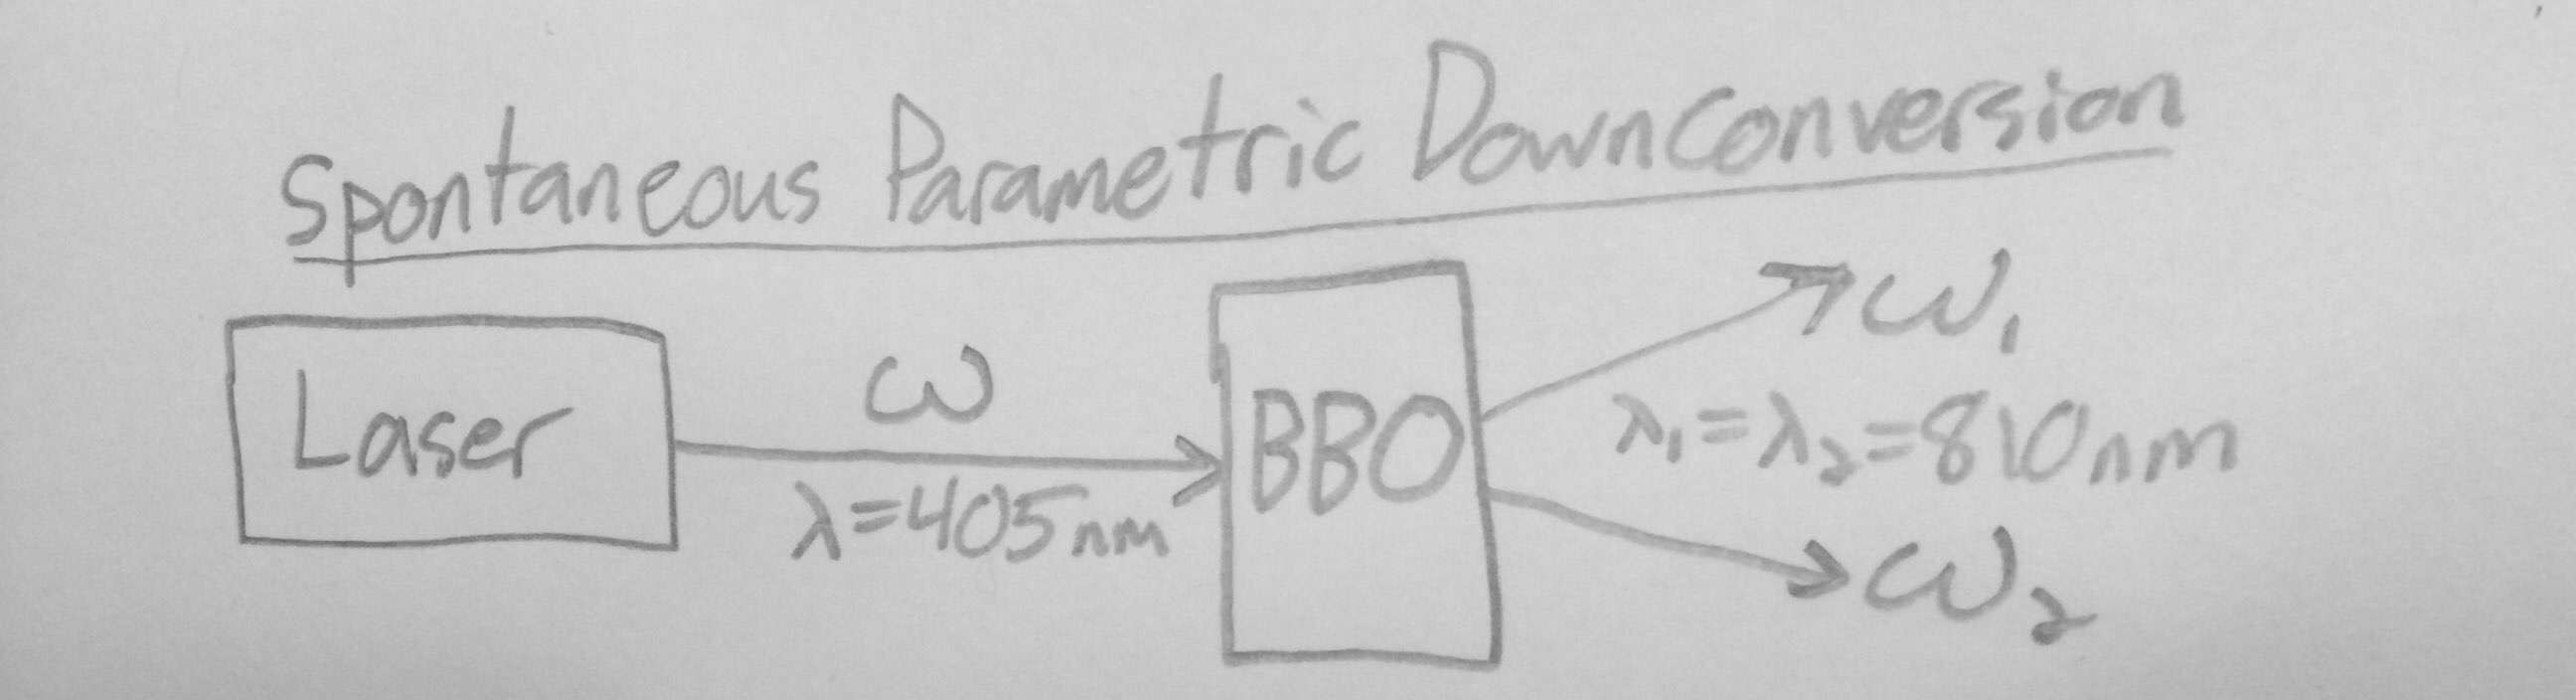
\includegraphics[scale = 0.15]{7.JPG}
    \caption{Visual Description of Spontaneous Parametric Downconversion}
    \label{fig:my_label}
\end{figure}
    The process, pictured above, is a result of the time-reversal of a process known as "sum-frequency generation (SFG)". SFG is essentially passing pairs of photons of different frequencies ($\omega_1$ and $\omega_2$) through nonlinear crystals that roughly function as ions with anharmonic potentials that, once driven by the photon pairs, oscillate at frequencies of linear combinations of $\omega_1$ and $\omega_2$, most notably $\omega_1 + \omega_2$. Ions irradiate at the sum frequency $\omega_1 + \omega_2$, among others. Because SPD necessitates a time-reversal of SFG, we see that incoming light at frequency $\omega$ is broken down into pairs of photons of frequency $\omega_1$ and $\omega_2$. For the purposes of this experiment, the wavelength $\lambda$ of the incident pump beam is 405nm, while the wavelengths of both of the two downconverted photons are 810nm, enabling the proper summing of the frequencies to that of the original pump photon. \cite{deh} 
    
    The BBOs used in this experiment are unique in that they only downconvert photons of a certain polarization. The first BBO downconverts the horizontal polarization of the photon, while the second BBO downconverts  vertical polarizations, such that the vertical polarization is allowed to pass through the first BBO unchanged until it reaches the second– the separation is so small that this happens nearly instantaneously. The downconversion process also works in such a way that the polarization of the two emerging downconverted photons are orthogonal to the polarization of the pump/incoming photon, via the following relationship (note: DC = downconverted) \cite{deh}:
    \begin{equation}
        \begin{array}{c}
            \ket{V_{pump}} \rightarrow \ket{HH_{DC}}\\
            \ket{H_{pump}} \rightarrow e^{i\delta}\ket{VV_{DC}}
        \end{array}
    \end{equation}
    where offset phase $\delta$ is an artifact of the crystal geometry and its resulting dispersion. Applying the BBOs to the pump photon ($\ket{\psi_{pump}}$) produced above, we yield the following quantum state coming out of the BBO that describes the two emerging photons:
    \begin{equation}
        \ket{\psi_{DC}} =  cos\theta_l\ket{HH_{DC}} + e^{i(\phi_l + \delta)}sin\theta_l\ket{VV_{DC}}
    \end{equation}
    which is already an entangled state. Directions in the procedures section will tell you how to directly construct the aforementioned $\ket{\psi_{EPR}}$ state, but essentially, we want to find a way to set $\theta_l$ to $45\degree$ and $\phi_l$ to $-\delta$.
    \\\indent That aside, we can motivate Bell's inequality and explain what mechanisms we will use to violate it by utilizing and measuring $\ket{\psi_{DC}}$. First, for the entangled photon pairs emerging from the BBO, we call the first photon the "signal" photon and the second the "idler" photon, and due to conservation of momentum, the two photons leave the BBO on paths that are a few degrees off from the pump state path direction, the photon pairs taking opposite perturbed deviations from the path. By measuring the polarization of the signal photon of $\ket{\psi_{DC}}$ in a the original basis rotated by $\alpha$ and the idler in a basis rotated by angle $\beta$ (measurement done by seeing probability that state was in $\ket{V}_\alpha\ket{V}_\beta$ = $\ket{V_\alpha V_\beta}$), we see that the probability of measuring the signal and idler as vertical in $\alpha$ and vertical in $\beta$, $P_{VV}(\alpha,\beta)$ is:
    \begin{equation}
        P_{VV}(\alpha,\beta) = |\bra{V_\alpha V_\beta}\ket{\psi_{DC}}|^2 = sin^2\alpha sin^2\beta cos^2 \theta_l + cos^2\alpha cos^2\beta sin^2 \theta_l + \frac{sin(2\alpha) sin(2\beta)cos(2\theta_l)cos(\phi_l + \delta)}{4}
    \end{equation}
    when using the following rotation of basis \cite{deh}:
    \begin{equation}
        \begin{array}{c}
        \ket{H_\alpha} = sin\alpha \ket{V} + cos\alpha \ket{H}\\
            \ket{V_\alpha} = cos\alpha \ket{V} - sin\alpha \ket{H}
        \end{array}
    \end{equation}
    Because of the finite line width of our pump light, $\phi_l + \delta$ varies over time, so we can time average this in our final experimental apparatus. When our downconverted state is $\ket{\psi_{DC}} = \ket{\psi_{EPR}} = \ket{\Phi^+}$, we see that this probability reduces to: \begin{equation}
        P_{VV}(\alpha,\beta) = \frac{cos^2(\beta - \alpha)}{2}
    \end{equation}
    For any pair of downconverted photons, we can measure the outcome of getting, along with outcome $V_\alpha V_\beta$, outcomes $H_\alpha V_\beta$, $V_\alpha H_\beta$, and $H_\alpha H_\beta$ by replacing $V_\alpha V_\beta$ in the above $P_{VV}$ expression.
    
    In order to test Bell's inequality, we introduce two correlational measures, $E(\alpha,\beta)$ and S, where:
    \begin{equation}
        E(\alpha,\beta) \equiv P_{VV}(\alpha,\beta) + P_{HH}(\alpha,\beta) - P_{HV}(\alpha,\beta) -  P_{VH}(\alpha,\beta)
    \end{equation}
    which describes the degree by which the polarizations for the signal and idler agree \cite{deh}. S, though less physically meaningful, is: 
    \begin{equation}
        S \equiv E(a,b) - E(a,b') + E(a',b) + E(a',b')
    \end{equation}
    for four polarizer angles a, a', b, b'. It was proved by Clauser, Horne, Shimony and Holt (CHSH) that if the correlates were indeed influenced by local hidden variables, that:
    \begin{equation}
        |S^{(HVT)}| \leq 2
    \end{equation}
    which is Bell's inequality, which we hope to violate. The proof essentially boils down to the fact that via HVT, we assume no entanglement and such that the probability of measurement of one photon does not depend on the measurement of the other. Thus, $E(\alpha,\beta)$ becomes $A_{\alpha}*B_{\beta}$ (with averaging over a distribution of hidden variables omitted for simplification of the problem). S thus becomes S = E(a,b) - E(a,b') + E(a',b) + E(a',b') = $A_a B_b - A_a B_{b'} + A_{a'} B_b + A_{a'} B_{b'}$ = $A_a( B_b - B_{b'}) + A_{a'}(B_b + B_{b'})$, where each value ($A_a, B_b$, etc.) can take on values +1 for vertical detection and -1 for horizontal detection in the relevant basis, and we see that S can only take on values $\pm 2$, and with integration over hidden variables, we recover Bell's inequality. \cite{bell}\cite{qie} % Include what results would be like for an EPR pair and QM results
    
    \indent For the quantum mechanics treatment, we see that $E(\alpha,\beta)$, when $P_{VV}, P_{HV}, P_{VH}, P_{HH}$ are fully expressed, essentially is the probability that the polarizations of the photon pair agree minus the probability of disagreement, and for the $\ket{\psi_{EPR}}$ state, this is:
    \begin{equation}
        E(\alpha,\beta) = cos^2(\beta - \alpha) - sin^2(\beta - \alpha)
    \end{equation}
    and plugging this into the defined expression for S(a,a',b,b'), and maximizing the multivariable expression S with polarizer angles a, a', b, b', we see that the maximum value for S that can be achieved is $2\sqrt{2}$ for angles $a = −45\degree,a' = 0\degree,b = -22.5\degree$ and $b' = 22.5\degree$. This requires that the downconverted photon pair is in state $\ket{\psi_{EPR}}$ and the angles are as such. If the angles vary from the maximization angles, or the state is other than $\ket{\psi_{EPR}}$, the following relationship holds true:
    \begin{equation}
        S^{(QM)} \leq 2\sqrt{2}
    \end{equation}
    which is a violation of Bell's inequality. The importance here is that if we are able to measure an S value such that S is greater than 2, then we would have violated Bell's inequality, and shown that local hidden variables are not an accurate description for this phenomenon. Showing S $>$ 2 demonstrates that Quantum Mechanics is a valid theory for nature and disproving any local hidden variables \cite{deh}\cite{qie}\cite{bell}.
    \\\indent In this experiment, each photon in the downconverted photon pair is passed through a half-wave plate and a beamsplitter that performs a unitary rotation of each photon's polarization and transmits remaining vertically polarized light through the splitter and into a detector. The combination of these two devices has the effect of measuring each downconverted photon in a new basis described by the rotation of basis equation (eq. 9); they function as a polarizer. The probability of finding the photon pair as both vertical in the $\alpha$ and $\beta$ rotated bases, $P_{VV}$, was given by equation 8. To actually measure $P_{VV}$, we measure the coincidence count of the number of photon pairs that both vertical in $\alpha$ and $\beta$ bases and divide that by the total number of coincident photon pairs that have both $V_\alpha V_\beta$,  $H_\alpha V_\beta$, $V_\alpha H_\beta$, and $H_\alpha H_\beta$ outcomes. To measure something as $H_\theta$ in some rotated basis, where $\ket{V_\theta}$ is $\theta$ degrees from the original vertical $\ket{V}$, we simply rotate the polarizer such that the new polarization, $\ket{H_\theta}$, is perpendicular to $\theta$, that is, $\theta + 90\degree$. We can say that this new measurement we are making is $H_\theta = V_{\theta + 90\degree}$, which we can also denote as $V_{\theta_\bot}$. Here $\theta_\bot$ = $\theta + 90\degree$, and all of this is described via the following figure: 
    \begin{figure}[H] %FIX
    \centering
    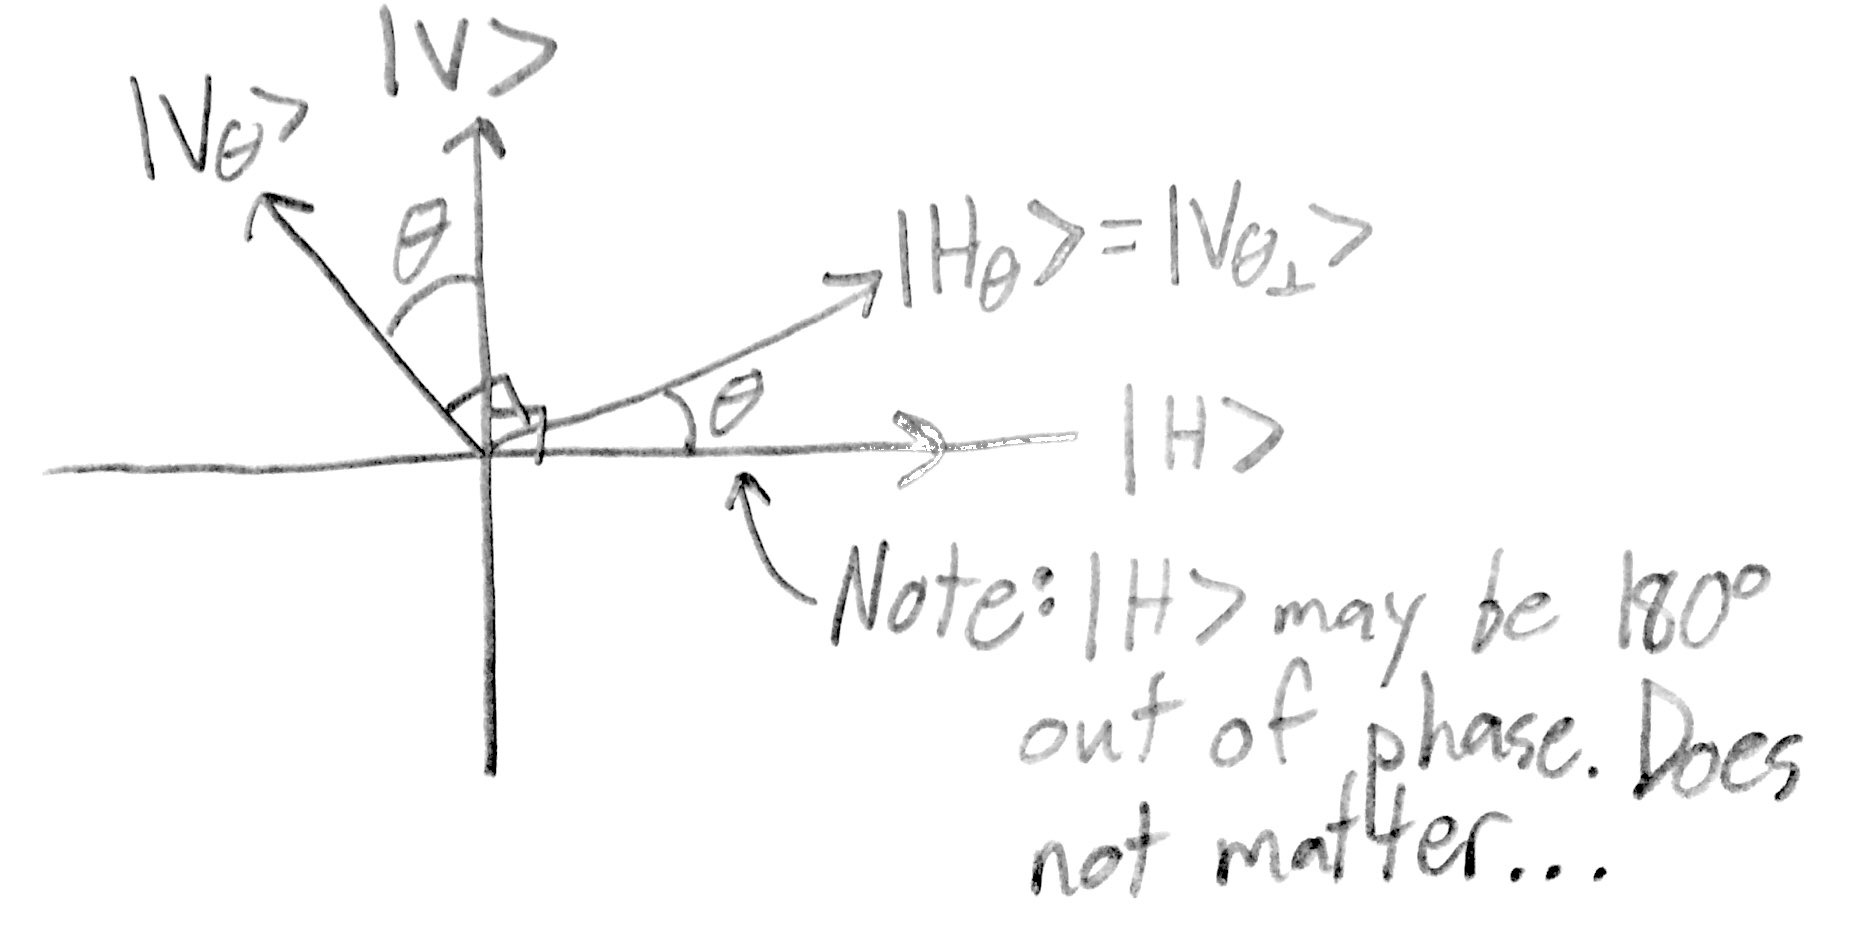
\includegraphics[scale = 0.15]{4.JPG}
    \caption{$\ket{H}$ and $\ket{V}$ rotated by angle $\theta$ to new basis $\ket{H} = \ket{V_{\theta_\bot}}$ and $\ket{V_\theta}$}
    \label{fig:my_label}
\end{figure}
    The following describes how to measure the probability of finding a photon pair in a certain bases for the VV, HH, VH and HV outcomes: 
    \begin{equation}
        P_{VV}(\alpha,\beta) = \frac{N(\alpha,\beta)}{N_{tot}}, 
        P_{HV}(\alpha,\beta) = \frac{N(\alpha_\bot,\beta)}{N_{tot}}, 
        P_{VH}(\alpha,\beta) = \frac{N(\alpha,\beta_\bot)}{N_{tot}}, 
        P_{HH}(\alpha,\beta) = \frac{N(\alpha_\bot,\beta_\bot)}{N_{tot}} 
    \end{equation}
    where $N_{tot}$, the total number of coincidences, is:
    \begin{equation}
        N_{tot} = N(\alpha,\beta) + N(\alpha_\bot,\beta) + N(\alpha,\beta_\bot) + N(\alpha_\bot,\beta_\bot)
    \end{equation}
    and $N(\alpha,\beta)$ is the number of photon pair coincidences when measuring the signal in $\alpha$ and the idler in $\beta$.
    So when we are measuring the number of coincidences for the signal and idler, for VV, we rotate the polarization of the incoming downconverted photon by $\alpha$ and $\beta$ respectively, beam split out horizontally polarized light, and detect remaining vertically polarized light (it does not matter which polarization is filtered out, all that matters is that it only allows one polarization to pass). For any H component we wish to measure (eg. $P_{HH}$), we rotate this polarization angle, $\alpha$ or $\beta$, by an additional 90$\degree$.\\\indent What do we mean by a coincidence? We define a coincidence event as when two photons hit a detector at the same time. Obviously, this is impossible to do due to the infinitesimally small path distance changes between the signal and idler, which would cause the signal and idler photons to arrive at their detectors at slightly different times. Thus, we allow a five nanosecond window for two photons to hit their detectors to be registered as a coincidence event. Typically (with a very high probability), these coincidence photon pairs are the signal and idler of the downconverted photon pairs. However, some of these coincidences may be accidental, resulting from effects such as ambient/background light passing into exposed detectors, the saturation of the photon pump beam producing too many downconverted pairs such that the time intervals of detection between alternate pairs overlap, reflections of the pump beam into the BBO that may also boost these rates, and a variation in this precise time window by electrical hardware. That aside, we can compute the statistic $E(\alpha,\beta)$ through the following method:
    \begin{equation}
        E(\alpha,\beta) = P_{VV}(\alpha,\beta) + P_{HH}(\alpha,\beta) - P_{HV}(\alpha,\beta) -  P_{VH}(\alpha,\beta) = \frac{N(\alpha,\beta) + N(\alpha_\bot,\beta_\bot) - N(\alpha_\bot,\beta) - N(\alpha,\beta_\bot)}{N_{tot}}
    \end{equation}
    and compute S as such through its dependence on $E(\alpha,\beta)$ in the aforementioned expression using four measurement angles ($\alpha, \beta, \alpha_\bot, \beta_\bot$) to find each $E(\alpha,\beta)$, and using angles a, a', b, and b' to find statistic S. We will make a total of sixteen measurements to account for all of these different polarizer angles (different basis rotations) \cite{deh}.
    \\\indent Furthermore, there exist various loopholes and assumptions in our experiment which may introduce hidden variables or cause us to find a lower value of S that could affirm HVT. We assume that axis of one of the BBOs is parallel to the beam splitter, and that the axes of the two BBOs are perpendicular to each other. We need to make this assumption in order to know how to construct the Bell State $\ket{\psi_{EPR}}$, which is detailed in the next section when we calibrate the angles of all of the half-wave plates. This may cause us to not actually produce a downconverted Bell state, which may cause us to record lower values for S. As aforementioned, background noise and dispersion and birefringence in the BBOs can decrease our S value. The effect of the BBOs essentially introduces elliptically polarized light to our linearly polarized pump beam. It is even likely that our input beam has some degree of circular polarization instead of initializing purely as horizontal, which has some effect on our downconverted state. 
    \\\indent A significant loophole in our experiment is the lack of spacelike separation between the signal and idler photon detectors. An important aspect of this experiment is the concept of causality. Suppose three people are simultaneously measuring the results of the experiment, of state $\ket{\psi_{EPR}}$. Two observers travel in opposite directions near the speed of light towards the two detectors along an axis formed by the detectors, while the last observer is stationary and the detectors are equidistant to him/her. An observer in the stationary frame will be able to detect the polarizations of the photons simultaneously, while observers in the equal and opposite moving frames will measure one particle before the other, depending on where they are coming from. Yet they all measure the same outcome, but the two travelling partners notice delays between the photons hitting the detector. We know as a prime function of quantum mechanics that wavefunction collapse occurs instantaneously after a measurement. From the viewpoint of each traveller, this appears to imply some sense of causality to the outcome of the second measurement, even though the coincidence is occurring simultaneously in the rest frame. We can reconcile the viewpoints of the observers because we know that although measurement of the first qubit can be random, the knowledge about the other qubit is transmitted at most at the speed of light, so in this sense, we have not violated causality. The notion of incorporating special relativity with instantaneous wavefunction collapse is important in closing a great loophole of the experiment, in which a causal relationship between the measurement of a photon and the measurement of another if it were to be affected by the first measurement could imply local hidden variables (i.e. believing that the measurement event of a photon from one perspective shaped the behavior of the other photon, perhaps by transmitting another photon between the two as an example of a hidden variable). We must demonstrate that entanglement holds true at nonlocal distances, for spontaneous wavefunction collapse can violate locality but not causality when it comes to the speed by which information can transfer. Essentially, if the two detectors were space-like separated, separated in such a way that a coincidence event would occur in less time than it would take light to travel between the two detectors, we would see that one detection could not possibly interfere with the other, and be able to absolutely refute HVT for this case. Sadly, the detectors for the signal and idler are placed closer than this, so we are presented with a caveat.
    \\\indent We discuss one more solution to the EPR paradox. The density matrix of $\ket{\psi_{EPR}}$ is the same, regardless of rotation, and thus describes the main state. The density matrix does also describe the distribution of eigen quantum states. Einstein essentially wanted to show that measuring one qubit in one basis, and the entangled other qubit in the other basis is incompatible and contrary to the uncertainty principle. However, who are we to distinguish measurements of individual qubits in this state when the main entangled state itself, described by the same density matrix regardless of the basis, is indistinguishable? Because of rotational invariance, we can propose it to be a futile effort to try to distinguish between the two states and also what the states are composed of. We arbitrarily attribute some state to the first qubit after it is measured.
    \\\indent All of this is just background in the main aim of our experiment, to prove that S $>$ 2 and thus disprove local hidden variables theories. There are a lot of contradictions that are inherent in quantum mechanics, so it is important to pursue many of these questions to gain deeper insight on the quantum mechanical description of nature. We have a lot of tools along the way that will help us achieve this goal.
    
    %FINISH with special relativity, quantum computing, wrong with EPR using density matrix, S and local realism + philosophy
    Our group could not study the effect of the quantum eraser because the previous lab group broke the laser we are using for this lab, so our group has been placed under significant time constraints. Theory behind the eraser is omitted. In the appendix, we have also included some notes on the application of this experiment to quantum computing.
    %we can measure the probability of finding the photon pairs in certain bases by counting the total number of photons that whose polarizations allow them to pass through rotated bases, to be described in the apparatus and procedures. The photons that pass through the rotated bases and are measured by detectors satisfy the $V_\alpha V_\beta$,  $H_\alpha V_\beta$, $V_\alpha H_\beta$, and $H_\alpha H_\beta$ outcomes. % add number of counts to here and explain coincidences and E(a,b) and why perpenticular for H condition...
% address what was wrong with EPR using density matrix
    %https://arxiv.org/pdf/quant-ph/0205171.pdf
    % http://users.unimi.it/aqm/wp-content/uploads/CHSH.pdf
    % https://arxiv.org/pdf/quant-ph/0205171.pdf
    % Half-wave plate description and why rotate for alpha and beta to get H alph and V alph, assumption BBO perp,
    % probabilities this way we make the assumption that the flux of photon pairs is the same in each interval and does not depend on the polarizer settings. These assumptions are reason- able, but they do create a “loophole” in our experimental test.
    % loophole of light travelling
    % loophole of background noise
    % what a coincidence is
    % false rates
    % circularly polarized light

\section{Apparatus and Procedure}
    \begin{figure}[H] %FIX
        \centering
        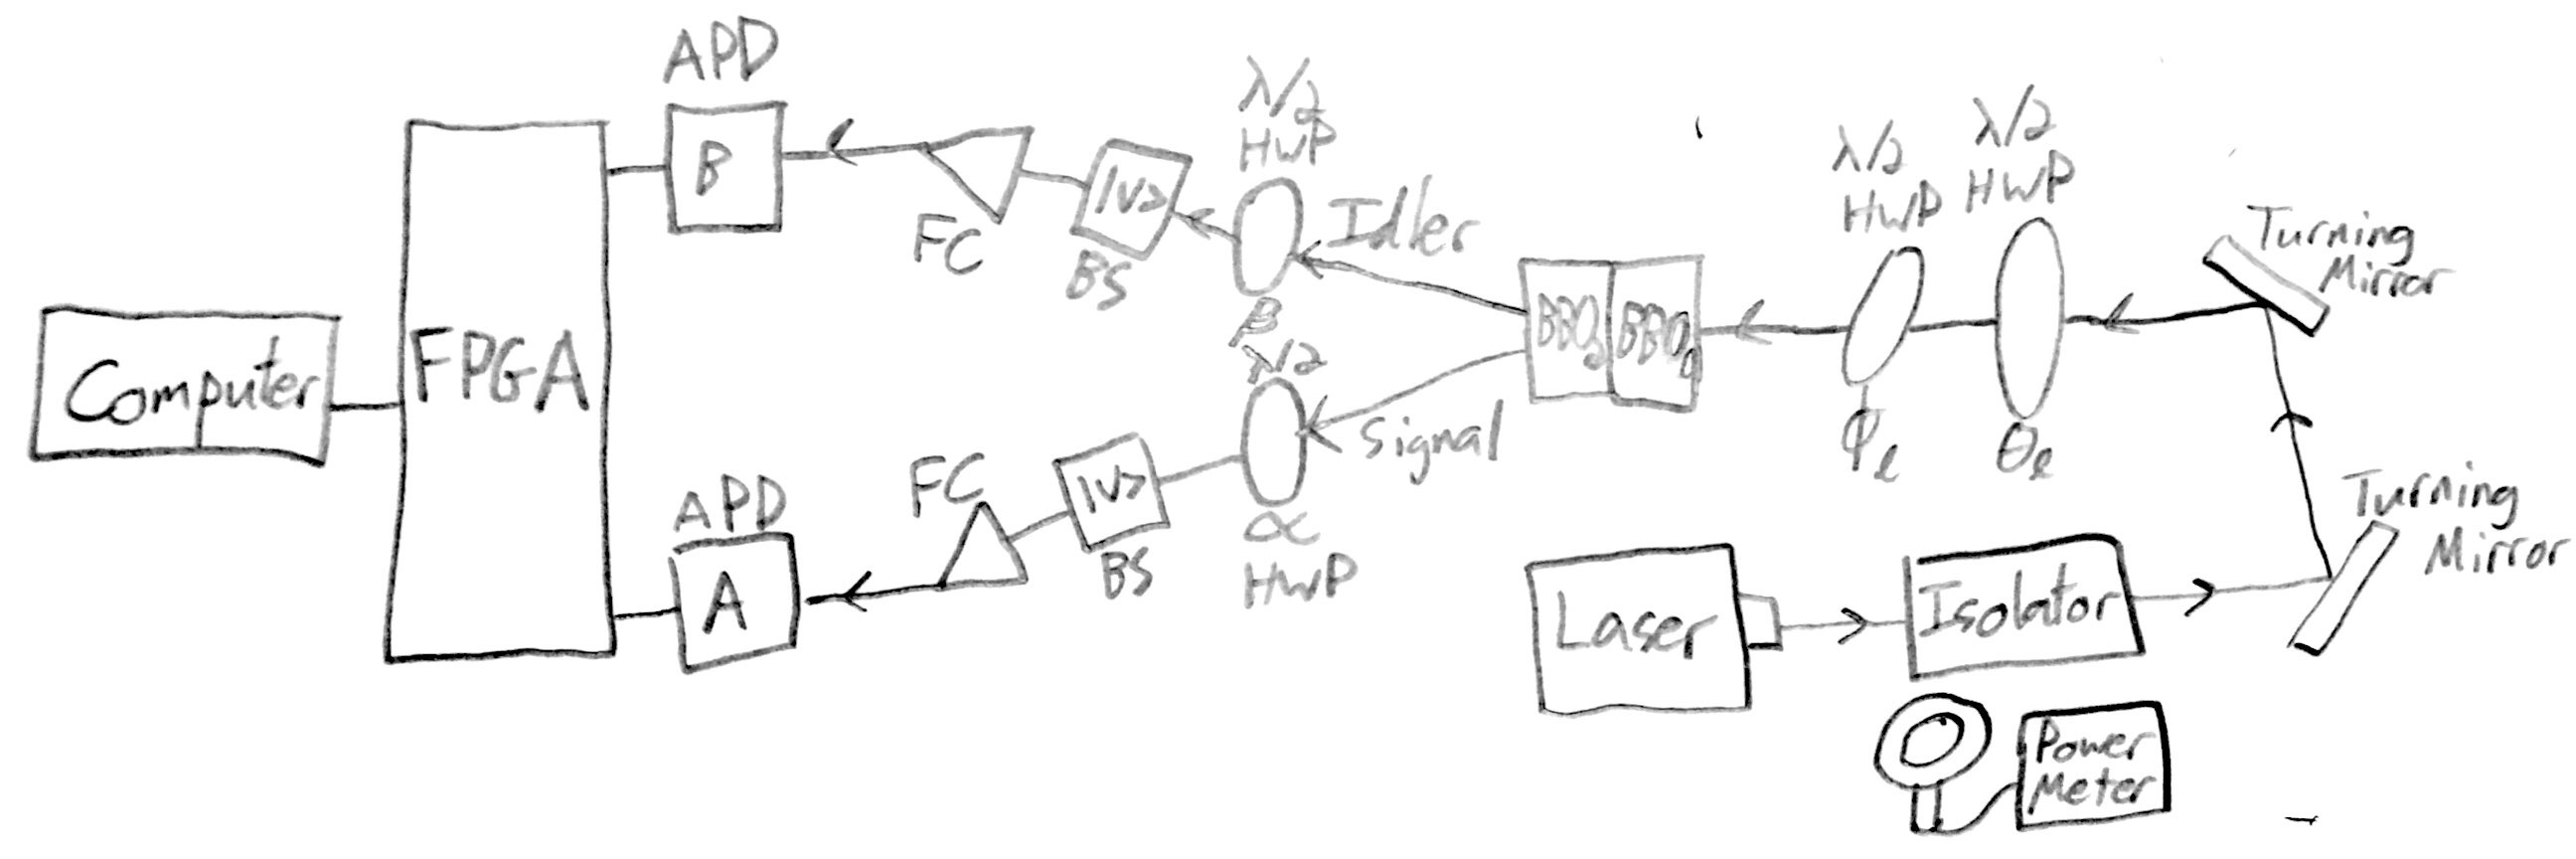
\includegraphics[scale = 0.2]{6.JPG}
        \caption{Diagram of Experimental Apparatus}
        \label{fig:my_label}
    \end{figure}
    % assume 
    Pictured above is a diagram of the experimental apparatus. Here we will quickly describe some of the equipment used to conduct this experiment:
    \begin{itemize}
        \item Diode laser- generates a 405 nm violet horizontally polarized photon beam to use in our experiment; has power supply control. There is a temperature controller that must be on as the laser diode is on.
        \item Optical isolator- prevents light from reflecting back into the laser diode. The previous lab group failed to incorporate this important element in the procedures and caused irreversible damage to the laser (hence our time-constraints in working on this lab).
        \item Turning mirrors- directs the beam from the isolator towards the BBOs.
        \item 405nm Half-Wave ($\lambda/2$ or HWP) Plates- Rotates the linear polarization of any incident photon, essentially transforming the basis of measurement for the photon's polarization. A half-wave plate is made out of a birefringent crystal that essentially reflects the polarization of a photon about some preferred/optical axis. A figure below explains this effect:  \cite{qie}
        \begin{figure}[H] %FIX
    \centering
    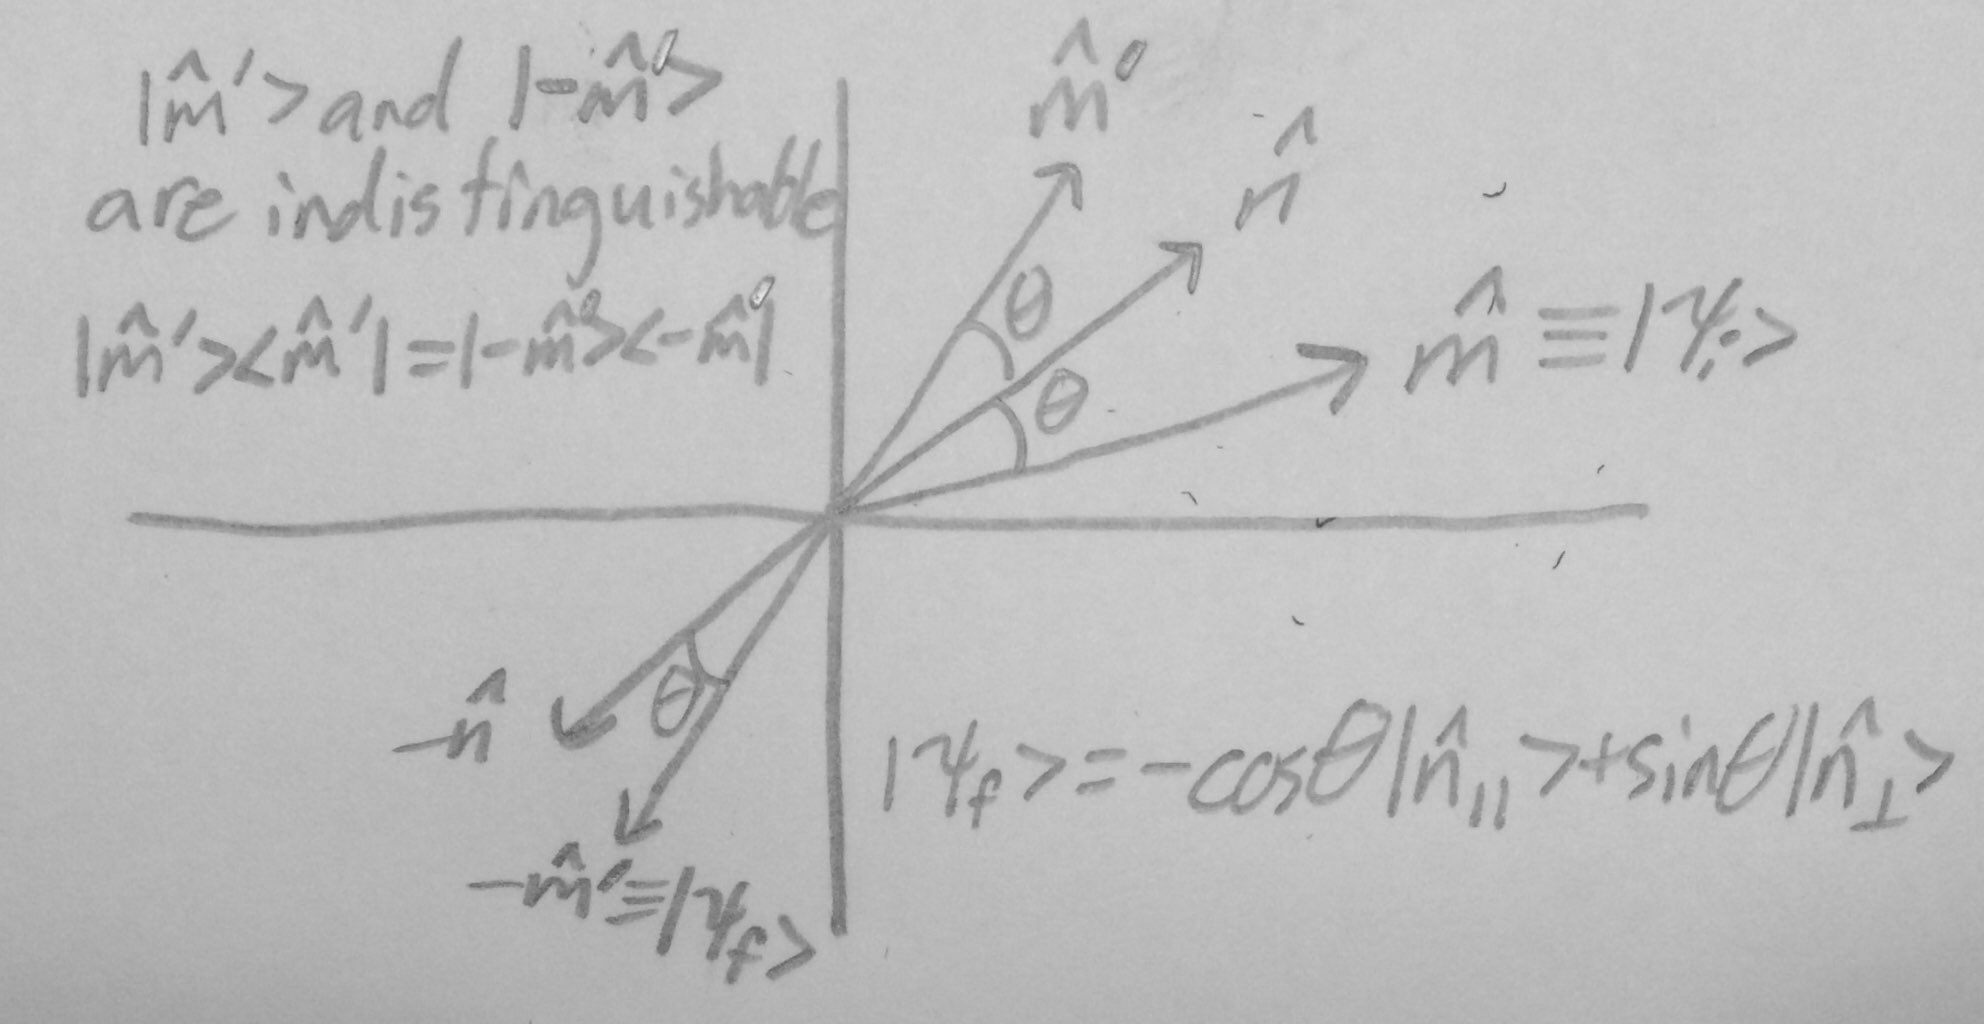
\includegraphics[scale = 0.15]{3.JPG}
    \caption{How the half-wave plate causes rotation of polarization by $2\theta$, where $\hat{n}\cdot \hat{m}=cos(\theta)$}
    \label{fig:my_label}
\end{figure}
        We see by this figure that the original polarization of the photon is $\hat{m}$, which does have some projection on the true horizontal and vertical axes, however, it also has a projection and perpendicular component along a preferred optical axis $\hat{n}$. We define the polarization of the photon as qubit $\ket{\psi_i} = cos\theta \ket{\hat{n_\parallel}} + sin\theta \ket{\hat{n_\bot}}$, where $\hat{n_\parallel}$ and $\hat{n_\bot}$ are parallel and perpendicular components of $\hat{n}$. The half-wave plate has the effect of changing the sign of the parallel component such that the final polarization is $\ket{\psi_f} = -cos\theta \ket{\hat{n_\parallel}} + sin\theta \ket{\hat{n_\bot}}$. If $\hat{m}$ is a $\theta$ degree rotation from $\hat{n}$, $\hat{m'}$ is what we hope to find, a $\theta$ degree reflection about $\hat{n}$ as described. When we applied $\lambda/2$ to the original qubit, the resulting polarization we found is $-\hat{m'}$. The qubit representative of this state $\ket{\psi_f}$, is indistinguishable from the qubit representing polarization $\hat{m'}$, if we were to take a look at the density matrices of the two states ($\ket{\hat{m}'}\bra{\hat{m}'}=\ket{-\hat{m}'}\bra{-\hat{m}'}$). So we say that we have used $\lambda/2$ to change the polarization of $\hat{m}$ by reflecting it about $\hat{n}$, by reflection angle $\theta$. Note that the optical axis that we set the half-wave plate to will perform a unitary rotation of angle $2\theta$, where $\theta$ is the angle between $\hat{m}$ and $\hat{n}$. \cite{qie} 
        \item Two BBOs- downconverts incident 405 nm photons into photon pairs of wavelength 810 nm, as described in the theory section. This generates our entangled downconverted photon pair state.
        \item Polarizing Beam Splitter Cube (BS)- Allows vertically polarized light to pass through but will reflect horizontally polarized light out at $90\degree$. This allows us to distinguish horizontally polarized light from vertically polarized light as we measure. 
        \item Fiber Coupler Lens (FC)- Focuses light onto a fiber optic cable.
        \item Avalanche Photo Diode (APD)- Converts photons into voltage. The APDs can be overloaded with high energy, so we take necessary precautions to prevent this.
        \item Field-programmable gate array (FPGA)- Takes signal from APDs and uses it to calculate the number of coincidences (coincidence count) between photon pairs hitting two detectors within a short (5 ns) interval, which can be programmed by the computer. To describe this short interval, every time a photon hits one detector, the FPGA waits 5 ns for the other photon in the pair to hit the other detector, and the event is registered as a coincidence. The data from the FPGA is sent to a computer.
        \item Computer- Receives data from the FPGA and allows us to take data on coincidence count rates as well as the photon count for each detector. We read the values (which can be time averaged) off of LabView interface, values of which we can use to calculate S.
        \item Long-pass filter- Protects eyes from laser radiation damage from violet light as well as protecting the APDs from overloading. Not pictured in diagram, but there is one to the left of the BBO, and two others to the right of the FCs.
        \item Red laser light (infrared laser)- Used for alignment of the optical equipment from the BBOs to the APDs.
    \end{itemize}
    The procedure for attaining our Bell State $\ket{\psi_{EPR}}$ using the equipment and finding S is outlined in the following steps. First, we provide a brief recap about theoretically how to generate a Bell State. Horizontally polarized light is generated by the laser diode, which after passing off the turning mirrors, passes through a half-wave plate, which ideally we can use to rotate the polarization of the 405nm photon to the $\frac{1}{\sqrt{2}}(\ket{H}+\ket{V})$ state. The photon is then passed through another half-wave plate, but this plate is able to rotate about its vertical axis, which introduces the complex phase factor $e^{\phi_l}$, as aforementioned, to the polarization. The photon then passes into the BBOs (and then the long pass filter), which should ideally downconvert the pump photon into 810 nm entangled photon pairs, as described in theory, which we hope are in a Bell State. The signal and idler photons then pass through another half-wave plate, which rotates the photons to their $\alpha$ and $\beta$ measurement bases. These photons pass through the polarizing beam splitter, and the photons that travel through will reach the APDs by FCs (protected by long pass filters) for detection via the FPGA. As previously mentioned, we use the coincidence counts for different half-wave plate basis rotations to help us deduce S.
    \\\indent In order to use this equipment, we must first align all of the optical elements so that the light can follow the correct path. To do this, we first aligned the optical elements from the laser diode to the BBOs with the help of the professor. We made slight adjustments to the angles of the turning mirrors and the height of some of the equipment such that the light that does not interact with the BBOs (before filtering the 405 nm light out with long pass filtering) is able to focus to a point in the center of a target located exactly between the detectors of the signal and idler photons. After turning on the laser diode and performing the alignment, we align the remainder of the optical equipment. Here we note that inserting the optical fibers into the APDs and red laser pointers, it is important to wiggle and not force the fiber into each port, else damage may occur. After removing long pass filters attached to the FCs and detaching the fiber optic cables from the APDs and attaching them to two red laser pointers, we shined infrared/red light through the optical cables such that red light would exit both FCs in the opposite path that light would normally travel in the experiment. This would allow us to trace the path of light through the second half of the apparatus, from the FCs to the BBOs. We removed the beam splitter and half-wave plates to first ensure the two light beams coming from the two FCs would focus on the BBOs opening, and we made small adjustments accordingly (height and rotation of FCs, adjusting screws on back of detector) until the two beams intersected on the BBOs' opening with the original violet pump beam. We reinserted and adjusted the height and rotation the half-wave plate and beam splitter cubes such that the two red light beams still converged at the BBOs' opening. We also made sure that red light passed through the center of the beam splitting cube (also reflecting into itself) and the same for half-wave plates (the plates are perpendicular to the light path's axis). Once this was done, we reinserted the long-pass filters and optical fibers into the APDs, shut off the lights, and turned on the diode laser, FPGA, and computer (to record coincidence counts). We further adjusted the optical elements to maximize coincidence counts to get a proper alignment.
    \\\indent The alignment being done, we moved on to other intermediate steps before measuring S. We checked the behavior of the laser diode by using a power meter to measure the output beam's power as we varied the current being supplied to the beam from 0mA to 100mA. The optical axis of the half-wave plates (to find what $\alpha$ and $\beta$ relatively are) is relatively unknown (some arbitrary offset from the true reading). We hope to find the optical axis where $\alpha,\beta=0\degree,0\degree$ ($0\degree$ means that the optical axis is vertical). From hereforth, we will denote the observed angle of the half-wave plates as $\alpha'$ and $\beta'$ respectively for the signal and idler photons' paths. We aim to calibrate $\alpha'$ and $\beta'$ such that $\alpha$ and $\beta$ are zeroed. First, we make the assumption that the transmission axis of the beam splitters (vertical) are parallel to one of the axes of the BBOs, when the two BBOs' axes are assumed to be perpendicular to each other, and we also assume the down-conversion efficiencies are similar between the BBOs. Then we remove the half-wave plates from the second half of the apparatus. We vary the first half-wave plate controlling $\theta_l$ (we also read its HWP angle as $\theta_l'$) until we are able to pass the horizontally polarized photon beam through the first HWP as a horizontally polarized pump beam. This would ensure that the beam is downconverted into two vertically polarized photon pairs, which could completely pass through the beam splitters and maximize the coincidence counts. After doing this, we reinsert the $\alpha$ and $\beta$ HWPs. If the optical axes of the HWPs are not aligned with the beam splitters, then the single counts and coincidence counts coming from each and both detectors would decrease. We adjust $\alpha'$ and $\beta'$ such that we maximize single and coincidence counts, and record these HWP angles. In this experiment, we see that $\theta_l' = 190\degree$ for maximum counts (corresponding to $\theta_l = 90\degree$) and the zeroes of the HWPs are $\alpha' = 273\degree, \beta' = 299\degree$.
    \\\indent Next, we needed to rotate $\theta_l$ and $\phi_l$ (its HWP reads $\phi_l'$) such as to produce the bell state. We found $\theta_l'$ such that $\theta_l = 45\degree$ by using a detuning method. It is expected that if we have a bell state, the number of coincidences, $N(\alpha,\beta)$, for angle pairs $\alpha,\beta$ = $0\degree,0\degree$ and $90\degree,90\degree$ ( $90\degree,90\degree$ corresponding to HWPs' angles $\alpha',\beta'=318\degree,344\degree$, $45\degree$ rotation of HWP because we only need to rotate half the angle of the polarization we hope to rotate too due to the nature of HWP) should be the same. That is, for a bell state, we would expect the coincidence count to be rotationally invariant, as the bell state is rotationally invariant. So we alternated our HWP angles between $\alpha,\beta = $ $0\degree,0\degree$ and $90\degree,90\degree$ and changed $\theta_l'$ as to equalize the counts between the two measurements (we measured angles around what we would expect for $\theta_l', 212.5\degree$). On the first day of measurement, we found this to be $\theta_l' = 210\degree$ and on the second day, it was $\theta_l' = 206\degree$. It is hard to explain why this change had happened. \cite{deh} Perhaps we had changed some of the alignment equipment when we checked alignment during different days; moving the table may have jostled some parts around. Maybe some of the connections that were holding the turning mirrors in place moved, or we removed and placed back the beam splitter, which may have had some bearing. Otherwise, perhaps the polarization of the incoming photon had changed from the other day when we had measured. This is all speculative, as we could not reach a consensus with other lab partners and the professor. It is true though that very small perturbations in the system could ultimately change the assumed downconversion rates between the two BBOs if the polarization of the pump beam had changed.
    \\\indent We tuned $\phi_l$ once $\theta_l$ was set appropriately. We set the HWPs at $\alpha,\beta = 45\degree,45\degree$ (when HWPs are rotated $22.5\degree$ from their $0\degree$ optical axis) and varied $\phi_l'$ until the coincidence count was maximized (see $P_{VV}$ equation), which was at $\phi_l' = 352.5\degree$ for both data collection days. That all being done, we measured the purity of the bell state on the second data collection day by recording values for $N(0\degree,0\degree),N(0\degree,90\degree),N(90\degree,90\degree),N(45\degree,45\degree)$, which will be used in the calculations section to find $C_1, C_2, \phi$ for $\ket{\phi_{DC}} = C_1\ket{HH} + C_2 e^{i\phi}\ket{VV}$ for $\phi = \delta+\phi_l$, where we hope to find $C_1=C_2=\frac{1}{\sqrt{2}}$ and $\phi = 0$. 
    \\\indent After ensuring that we constructed a pure bell state, we ran one more test before measuring S. We held $\alpha$ fixed at angles $0\degree, 45\degree,90\degree,$ and $135\degree$, corresponding to $\alpha'$ of $273\degree,295.5\degree,318\degree,340.5\degree$ respectively, and varied $\beta$ from $0\degree$ to $180\degree$ in equal-sized increments for each $\alpha$, and recorded data for four plots of coincidence count rates. We expect the plots to look sinusoidal, reflecting the change in measurement basis as measured by the projection of the downconverted photon pairs into this basis, essentially $P_{VV}$.  
    \\\indent Afterwards, we began to measure coincidence counts at various angles to find S, as detailed in the theory section. We made sixteen measurements, capturing four measurements for each $E(\alpha,\beta)$. For each $E(\alpha,\beta)$, we recorded coincidence counts $N(\alpha,\beta), N(\alpha,\beta_\bot), N(\alpha_\bot,\beta),$ and $N(\alpha_\bot,\beta_\bot)$, corresponding to $V_\alpha V_\beta, V_\alpha H_\beta, H_\alpha V_\beta,$ and $H_\alpha H_\beta$ respectively. We performed these sixteen total measurements for angle pairs (a,b), (a',b), (a,b'), and (a',b') for angles $a = -45\degree (\alpha' = 250.5\degree), a' = 0\degree (\alpha' = 273\degree), b = -22.5\degree (\beta' \approx 288 \degree)$ and $b' = 22.5\degree (\beta' \approx 310\degree)$.
    \begin{figure}[H] %FIX
    \centering
    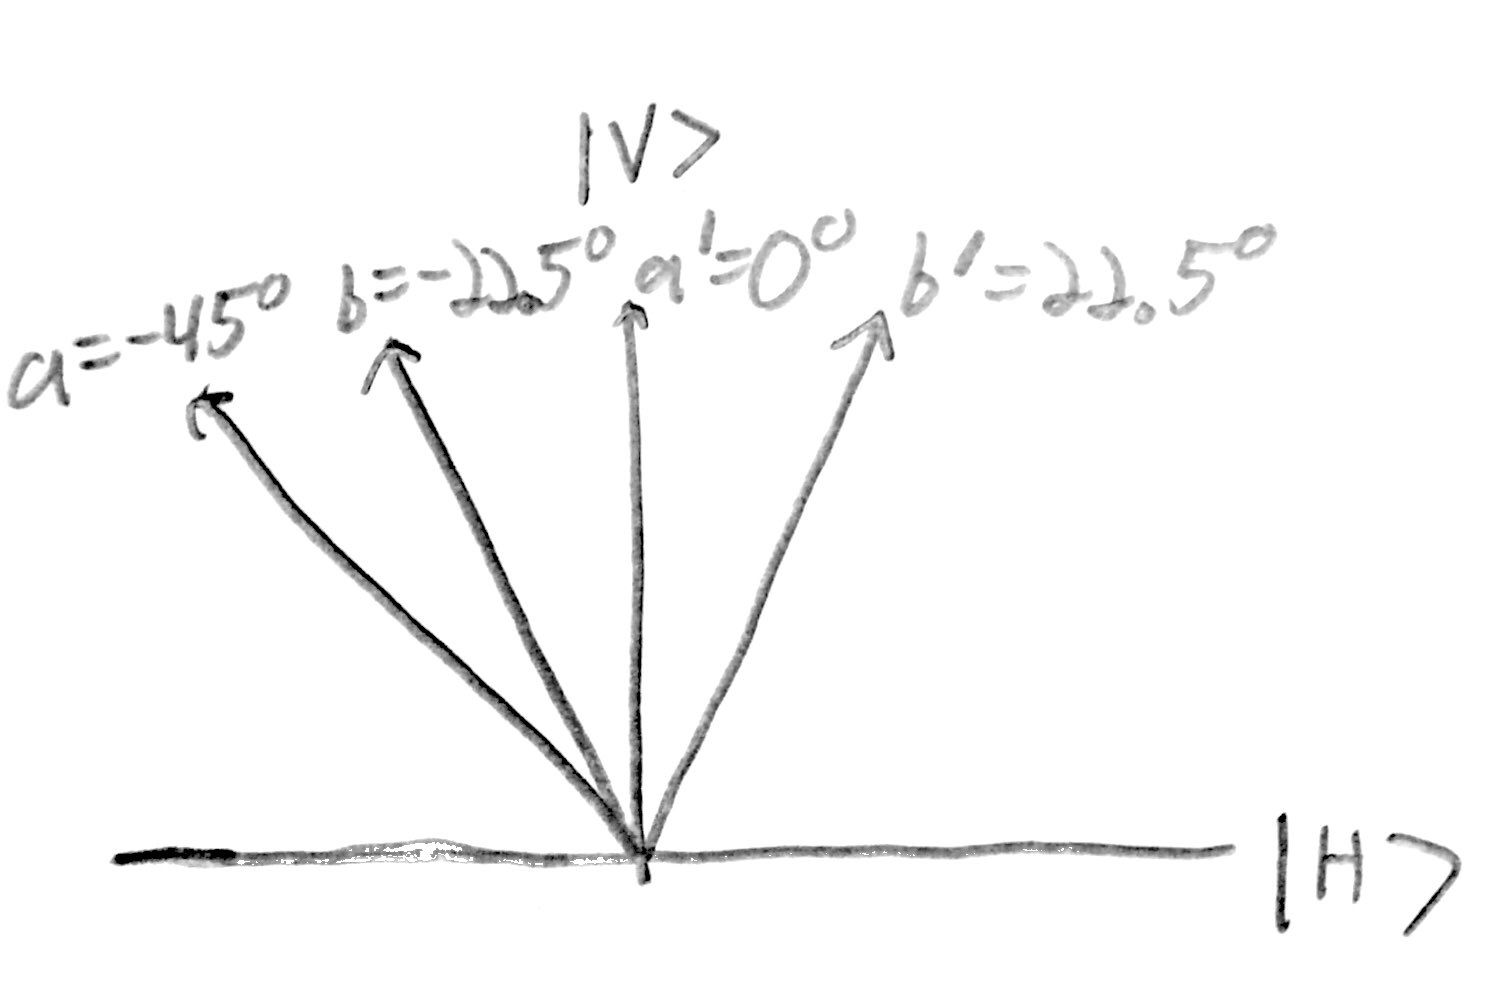
\includegraphics[scale = 0.15]{5.JPG}
    \caption{Polarization settings we will use to measure S, corresponding to the HWP readings $\alpha'$ and $\beta'$ listed above}
    \label{fig:my_label}
\end{figure}
    We rotated the HWPs to the appropriate angles, measured coincidence counts for a time of 10 seconds for each measurement, and recorded the data using LabView.
   
    NOTE: As we performed these measurements and calibrations, we actually looked at the coincidence count rates instead of the total counts, which is only off by a multiplicative timed constant factor. We also recorded coincidence counts for 10 seconds at a time to produce these time averaged coincidence rate values. Also, all HWP measurements made ($\theta'$) have an error $\sigma_{\theta'}$ of $\pm1\degree$, as the measurement error is half that of the number of degrees per division on the HWP readings. For our measurements, we also set the current of the laser diode to 36.17 mA.

\section{Calculation and Data Analysis}
    Produced below is a plot of the current fed into the violet laser diode versus the power of the laser diode beam found after the optical isolator (from table 1). 
    \begin{figure}[H] %FIX
    \centering
    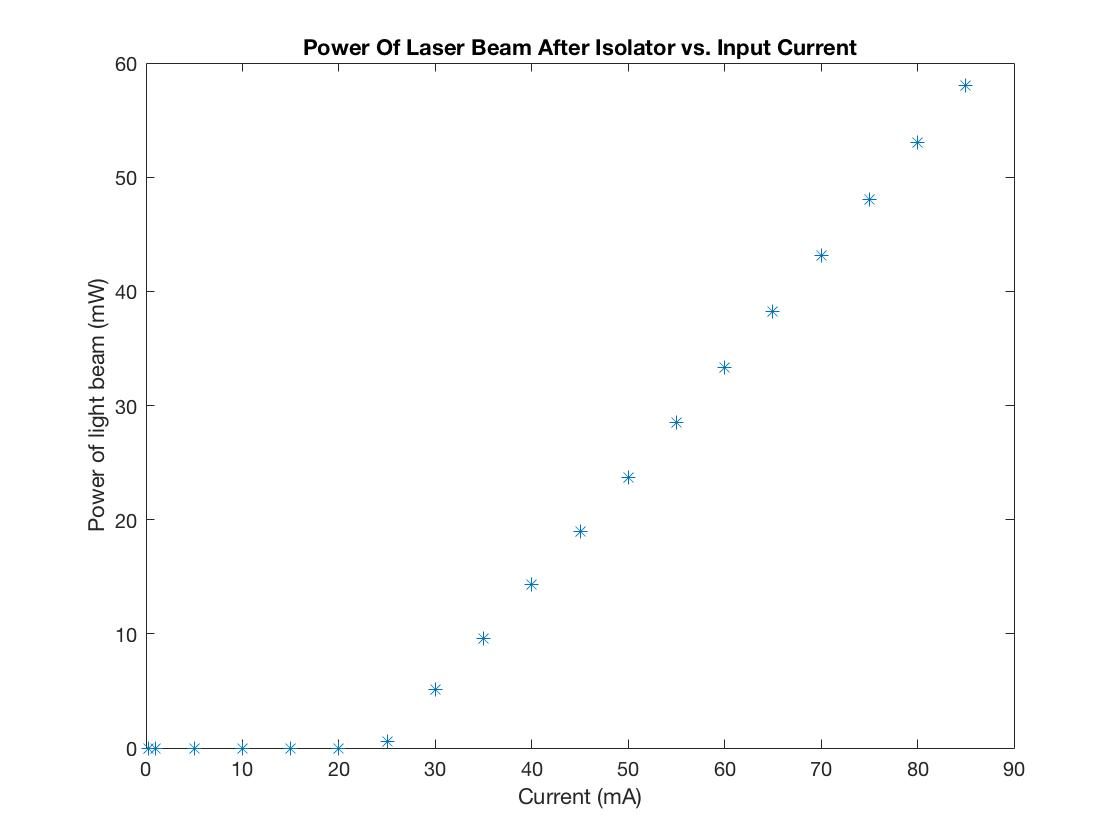
\includegraphics[scale = 0.3]{1.jpg}
    \caption{Plot of Current versus Power of Violet Laser Diode Beam (after isolator for power measurement)}
    \label{fig:my_label}
\end{figure}
     Here, we note that the laser does not begin generating power until it reaches a certain threshold. However, after this threshold, the curve appears to look linear, so the laser is working properly.
    \\\indent In our calculations, we may calculate the error in coincidence count rates, the number of coincidences per second. We will denote this rate as $N(\alpha,\beta)$, using N as before, but this time we change the denotation from total coincidences to a coincidence rate. The error for a total number of coincidences, the total number and error denoted as $\hat{N}$ and $\sigma_{\hat{N}}$ respectively, is $\sigma_{\hat{N}} = \sqrt{\hat{N}}$, under the assumption that a distribution of the total number of coincidences follows a Poisson distribution. The coincidence rate is N and its error $\sigma_N$ is equal to $\frac{\sqrt{N*\Delta T}}{\Delta T} = \sqrt{\frac{N}{\Delta T}}$, where $\Delta T$ is the total time of acquisition of coincidences. 
    \\\indent We already measured the zeroed HWP angles, noting measurement errors of $1\degree$. Data for finding $\theta_l'$ and $\phi_l'$ is outlined in the Raw Data section. Judging by table 2, we see that for days one and two, $\phi_l'$, with a maximum coincidence count rate of 713.3, was found to be $352.5\pm 1\degree$. For day one, $\theta_l'$ was found to be $210\degree\pm 1\degree$, and for day two, it was $206\degree \pm 1\degree$. 
    \\\indent We explored the dependence of the coincidence rates as related to the settings on the HWPs attached to the detector arms in order to conduct a preliminary test on the purity of the bell state. As aforementioned, holding $\alpha$ fixed at $45\degree$ increments and varying $\beta$ in 10$\degree$ increments, we should expect to observe a sinusoidal curve as depicted in our equation for $P_{VV}$. The data set is large (table 4) and has been included in the raw data section. We plot the coincidence rates with error bars below for varying $\beta$ values and fixed $\alpha$ values (after converting HWP angles into $\beta$ angles):
 \begin{figure}[H] %FIX
    \centering
    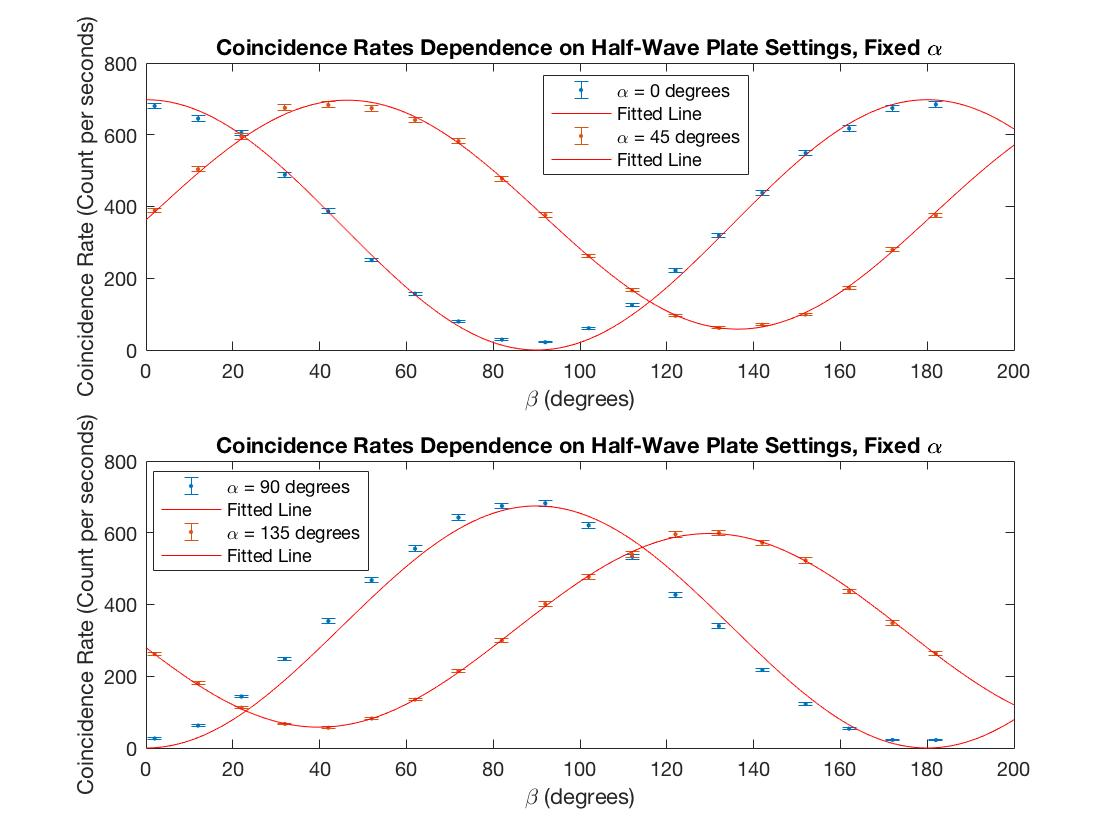
\includegraphics[scale = 0.3]{2.jpg}
    \caption{Coincidence rates as a function of $\beta$ for fixed $\alpha$, after conversion from particular HWP angles}
    \label{fig:my_label}
\end{figure}
    \indent We performed a weighted fit \cite{err} (equation from Taylor, using $\sigma_{N_i}^{-2}$ as the $i^{th}$ weight, see next paragraph) to each data set using the function $N_{VV}(\beta) = N*P_{VV}(\beta)$ for fixed alpha. That is, we used $N_{VV}(\beta)_\alpha = N*|\bra{V_\alpha V_\beta}\ket{\psi_{DC}}|^2 = N*(C_1^2sin^2(\beta)sin^2(\alpha)+C_2^2sin^2(\beta)sin^2(\alpha)+\frac{C_1*C_2*sin(2\beta)sin(2\alpha)*cos(\phi)}{2})$ for $\ket{\psi_{DC}} = C_1\ket{HH} + C_2e^{i\phi}\ket{VV}$ with all parameters being fit parameters ($N,C_1,C_2,\phi$) except $\beta$ and $\alpha$. We plotted the fits with their corresponding data, and found very high correlational adjusted r-squared values for each fit. For the cases where $\alpha$ was fixed to $0\degree,45\degree,90\degree,135\degree$, we found adjusted r-squared values of 0.9852, 0.9988, 0.9611, and 0.9995, respectively (fifteen degrees of freedom). This means that most (at least $96\%$) of the variation in the data could be explained by the model. In this case we see that the dependence of the coincidence rate as a function of HWP settings corresponds to what we would expect, as inferred from a highly predictive model. We calculated a reduced Chi-Squared value for each fit from the equation:
    \begin{equation}
        \tilde{\chi}^2 = \frac{\sum_{i=1}^{15}(\frac{N_i - N(\beta_i)}{\sigma_{N_i}})^2}{15}
    \end{equation}
    where 15 is the degrees of freedom for each fit, $\sigma_{N_i}$ is the expression in the next paragraph, $N_i$ is the $i^{th}$ observed coincidence rate data point, and $N(\beta_i)$ is the point found from the fit for $\beta_i$. For the cases where $\alpha$ was fixed to $0\degree,45\degree,90\degree,135\degree$, resulting reduced Chi-Squared values were 38.569,  2.020, 96.298, and 0.757 respectively. The $\alpha = 45\degree$ and $135\degree$ fits were good models for the data, while the other two fits had their residuals a bit larger than the errors of each data point.
    \\\indent Now to measure the purity of the bell state itself. We hope to find $C_1,C_2,$ and $\phi$ such that $\ket{\psi_{DC}} = C_1\ket{HH} + C_2e^{i\phi}\ket{VV} = \ket{\psi_{EPR}}$. To do this, we used the directions specified by Dehlinger and Mitchell \cite{deh}, where we use our data points $N(0\degree,0\degree),N(0\degree,90\degree),N(90\degree,90\degree),N(45\degree,45\degree)$ with error $\sigma_N = \sqrt{\frac{N}{\Delta T}}$ (remember that N is now the coincidence count rate, $\Delta T$ is a 10 second acquisition time) in the following way:
    \begin{equation}
        C = N(0\degree,90\degree) \pm \sigma_{N(0\degree,90\degree)}
    \end{equation}
    \begin{equation}
        A = d_1 + d_2 - 2C
    \end{equation}
    \begin{equation}
        tan^2\theta_l = \frac{d_2 - C}{d_1 - C}, \theta_l = \arctan(\sqrt{\frac{d_2 - C}{d_1 - C}})
    \end{equation}
    \begin{equation}
        cos\phi = \frac{1}{sin(2\theta_l)}*(4*\frac{d_3 - C}{A} - 1), \phi = \arccos(\frac{1}{sin(2\theta_l)}*(4*\frac{d_3 - C}{A} - 1))
    \end{equation}
    where we denote:
    \begin{equation}
        d_1 \equiv N(0\degree,0\degree), d_2 \equiv N(90\degree,90\degree), d_3 \equiv N(45\degree,45\degree)
    \end{equation}
    We find propagated errors using the following expressions:
    \begin{equation}
        \sigma_A = \sqrt{\sigma_{d_1}^2 + \sigma_{d_2}^2 + 4*\sigma_C^2}
    \end{equation}
    \begin{equation}
        \sigma_{\theta_l} = \sqrt{(\frac{\partial{\theta_l}}{\partial{d_1}}*\sigma_{d_1})^2 + (\frac{\partial{\theta_l}}{\partial{d_2}}*\sigma_{d_2})^2 + ( \frac{\partial{\theta_l}}{\partial{C}}*\sigma_{C})^2}
    \end{equation}
    \begin{equation}
        \sigma_{\phi} = \sqrt{(\frac{\partial{\phi}}{\partial{d_3}}*\sigma_{d_3})^2 + (\frac{\partial{\phi}}{\partial{C}}*\sigma_{C})^2 + (\frac{\partial{\phi}}{\partial{A}}*\sigma_{A})^2 + (\frac{\partial{\phi}}{\partial{\theta_l}}*\sigma_{\theta_l})^2}
    \end{equation}
    where the last two expressions' derivatives were analytically computed using symbolic mathematical expressions via MATLAB, and then numerical values for each expression were computed using our data (table 3). This yielded results $A = 1.322*10^3 \pm 12. \frac{counts}{second}$, $\theta_l = 45.024\degree \pm 0.181 \degree$, and $\phi = 8.5233\degree \pm 9.108\degree$. We would expect that $\theta_l$ would equal $45\degree$ and $\phi = 0\degree$ for us to have produced a Bell State, and we see here that our expected $\theta_l$ and $\phi$ values fall within our experimental bounds for the measured values. Thus, we can say that this, in conjunction to the aforementioned highly predictive model of coincidence count dependence on HWP settings, means that we have a quite pure bell state. 
    \\\indent S, our final statistic, was computed using a familiar equation from the theory section:
    \begin{equation}
        S = E(a,b) - E(a,b') + E(a',b) + E(a',b')
    \end{equation}
    which expanded for $E(\alpha,\beta) = \frac{N(\alpha,\beta) + N(\alpha_\bot,\beta_\bot) - N(\alpha_\bot,\beta) - N(\alpha,\beta_\bot)}{N(\alpha,\beta) + N(\alpha_\bot,\beta_\bot) + N(\alpha_\bot,\beta) + N(\alpha,\beta_\bot)}$ looks like:
    \begin{equation}
    \begin{array}{c}
        S = \frac{N(a,b) + N(a_\bot,b_\bot) - N(a_\bot,b) - N(a,b_\bot)}{N(a,b) + N(a_\bot,b_\bot) + N(a_\bot,b) + N(a,b_\bot)} - \frac{N(a,b') + N(a_\bot,b'_\bot) - N(a_\bot,b') - N(a,b'_\bot)}{N(a,b') + N(a_\bot,b'_\bot) + N(a_\bot,b') + N(a,b'_\bot)} + \\\frac{N(a',b) + N(a'_\bot,b_\bot) - N(a'_\bot,b) - N(a',b_\bot)}{N(a',b) + N(a'_\bot,b_\bot) + N(a'_\bot,b) + N(a',b_\bot)} + \frac{N(a',b') + N(a'_\bot,b'_\bot) - N(a'_\bot,b') - N(a',b'_\bot)}{N(a',b') + N(a'_\bot,b'_\bot) + N(a'_\bot,b') + N(a',b'_\bot)}
        \end{array}
    \end{equation}
    where in this case we can still use coincidence count rates for N because all time measurements will cancel out, as they only add a constant multiplicative factor to the numerator and denominator of the equation. We can also relabel the N-values by the order in which they appear in the previous expression's numerators as $N_i$:
    \begin{equation}
        S(N_1,...,N_{16}) = \frac{N_1 + N_2 - N_3 - N_4}{\sum_{i=1}^4 N_i} -\frac{N_5 + N_6 - N_7 - N_8}{\sum_{i=5}^8 N_i}  +\frac{N_9 + N_{10} - N_{11} - N_{12}}{\sum_{i=9}^{12} N_i} +\frac{N_{13} + N_{14} - N_{15} - N_{16}}{\sum_{i=13}^{16} N_i} 
    \end{equation}
    we see that the propagated error on S is \cite{deh}:
    \begin{equation}
        \sigma_S = \sqrt{\sum_{i=1}^{16} (\frac{\partial{S}}{\partial{N_i}})^2*\sigma_{N_i}^2} = \sqrt{\sum_{i=1}^{16} (\frac{\partial{S}}{\partial{N_i}})^2*N_i}
    \end{equation}
    which was computed via MATLAB via the expression:
    \begin{equation}
        \sigma_S = \sqrt{(\vec{\bigtriangledown S_N} \odot \vec{\sigma_N})\cdot (\vec{\bigtriangledown S_N} \odot \vec{\sigma_N})} = ||\vec{\bigtriangledown S_N} \odot \vec{\sigma_N}||
    \end{equation}
    where $\odot$ is element wise multiplication between vectors $\vec{\bigtriangledown S_N}$ and $\vec{\sigma_N}$, with the two defined as:
    \begin{equation}
        \vec{\bigtriangledown S_N} = \begin{bmatrix}
        \frac{\partial{S}}{\partial{N_1}}\\\frac{\partial{S}}{\partial{N_2}}\\.\\.\\\frac{\partial{S}}{\partial{N_{16}}} 
        \end{bmatrix},\vec{\sigma_N} = \begin{bmatrix}\sigma_{N_1}\\\sigma_{N_2}\\.\\.\\\sigma_{N_{16}} \end{bmatrix},\vec{\bigtriangledown S_N} \odot \vec{\sigma_N} = \begin{bmatrix} \frac{\partial{S}}{\partial{N_1}}\sigma_{N_1}\\\frac{\partial{S}}{\partial{N_2}}\sigma_{N_2}\\.\\.\\\frac{\partial{S}}{\partial{N_{16}}}\sigma_{N_{16}} \end{bmatrix}
    \end{equation}
    Running this calculation via symbolic expression in MATLAB and inputting our N-values (coincidence count rates) for Day One of testing and day two (table 5), and we get $S_{day one} = 2.4855 \pm 0.0172$ and $S_{day two} = 2.4750 \pm 0.0179$. We see that both of these S-values are well above the upper bound of Bell's inequality, $S^{(HVT)}\leq 2$. Values found for S were between 2 and $2\sqrt{2}$.
    % ADD ACCIDENTAL RATE!@#$@#$!$%$#!^$


\section{Conclusion}
    %start conclusion here
    \subsection{Results and Discussion of Results}
    The goal of our experiment was to measure S such that it violates Bell's Inequality, allowing us to conclude that hidden local variables is not the correct model by which to view nature. To do this, we generated a horizontally polarized laser beam, and passed it through a complex optical system that would rotate its polarization to $\frac{1}{\sqrt{2}}(\ket{H} + \ket{V})$, eliminate any phase differences introduced by any elements, entangle photon pairs into $\ket{\psi_{EPR}} = \frac{1}{\sqrt{2}}(\ket{HH} + \ket{VV})$ by using a BBO to down convert 405 nm light with polarization  $\frac{1}{\sqrt{2}}(\ket{H} + \ket{V})$ to two 810 nm photons in the bell state. We would then pass the signal and idler photons of the pair into half-wave plates and polarized beam splitters to rotate and measure the photons in bases specified by $\alpha$ and $\beta$. We measured the coincidence count rates of the photon pairs as they struck their corresponding detectors in a small time interval. We first had to align the optical equipment such that light would pass through the system correctly from laser to detector. Then, after making sure the beam was outputting the proper amount of power, we followed a procedure that should have produced our bell state. We explored the dependence of the coincidence rates on the HWP settings and made additional measurements to test the purity of the bell state. Once we decided that the entangled state seemed to be a pure bell state, we went on to measure S by taking sixteen measurements of coincidence count rates at various specified HWP settings and analyzed the data to see whether we had violated Bell's inequality.
    \\\indent When calibrating all four HWPs (for expected values $\alpha = 0\degree,\beta = 0\degree, \theta_l = 45\degree, \phi_l = -\delta$), we found their corresponding HWP settings to be $\alpha'=273\pm 1\degree,\beta'=299\pm 1\degree, \theta_l' = 210\pm 1\degree$ (day 1), $\theta_l' = 206\pm 1\degree$ (day 2), and $\phi_l' = 352.5\pm 1\degree$. We attempted to measure the purity of our bell state on day two by first finding the dependence of coincidence counts on the $\alpha$ and $\beta$ HWP settings. We were able to produce a curve of $\beta$ versus coincidence counts that could be closely modelled by $P_{VV}(\alpha,\beta) = |\bra{V_\alpha V_\beta}\ket{\psi_{DC}}|^2$, and if we varied $\beta$ for four different fixed $\alpha$ angles. We attained correlational adjusted r-squared values above $96\%$ between the four curves for fixed $\alpha$ values of $0\degree,45\degree,90\degree,$ and $135\degree$, indicating that we had highly predictive models. For the same models, resulting reduced Chi-Squared values for the fits showed that half of the models fit the data well ($\tilde{\chi}^2\approx 1$), and the other two had slightly larger residuals than errors in the data points. We see that the data closely fit a model for what we would expect for $\ket{\psi_{EPR}}$. We were able to further test the purity of the state by measuring values for $\theta_l$ (expected value of $45\degree$) and $\phi = \delta + \phi_l$ ($0\degree$ expected value), which were measured to be $\theta_l = 45.024\degree \pm 0.181 \degree$, and $\phi = 8.5233\degree \pm 9.108\degree$. In this case, the expected values that generate the $\ket{\psi_{EPR}}$ state fell within our experimental bounds, so we conclude that we likely constructed a pure bell state.
    \\\indent With this information and measuring coincidence rates at various signal/idler HWP settings for S, we found S to be $S_{day one} = 2.4855 \pm 0.0172$ and $S_{day two} = 2.4750 \pm 0.0179$ over two separate trials. The two results violate Bell's Inequality, and thus we can conclude that local hidden variables theory is not an adequate description for nature. 
    \\\indent As discussion, it is necessary to point out that there is a lot of literature covering this matter and for how to reconcile EPR's paradox. In what we have just done in this experiment is experimentally point out fallacies in EPR's paper. It would appear that EPR's paradox is an artifact of a classical attempt to understand the measurement process of quantum mechanics, something that is truly a non-classical process. The measurement process of quantum mechanics is still a mystery to many and is still under interpretation. Dehlinger points out that the interpretation of quantum mechanics and measurement essentially two main spheres of thought, what some consider as the "many worlds" theorists, and then the Copenhagan interpretation (for the most part). HVT would have it that both localism (the ability for results to be dependent on the nearby environment) and realism (that a unique solution can be obtained given a set of circumstances) are valid assumptions for nature. However, as our experiment has shown, there is a tradeoff between these two assumptions: either localism is retained, or realism is retained, but neither can coexist. Most Copenhageners would postulate that when something is measured, spontaneous wavefunction collapse, instantaneous action at a distance violates locality, but a unique solution can be found for the particle's state/observable. Many worlds proponents would have it that locality can still be preserved if we believe that things are truly random, and no reality can ultimately explain why we are getting the results we are getting. In this sense, any solution is possible for a particular measurement, up to some probability \cite{deh}. It is an interesting debate between two camps of physicists. Personally, I believe in Copenhagen's interpretation, but it is understandable why the EPR paradox has enthralled physicists for the last few generations.
    
    \subsection{Some Possible Sources of Error}
    There are many possible sources of error in this experiment, though our conclusion, an S value well above 2, appears to maintain that we could minimize many of these confounding factors. However, our experimental result, found by setting the HWPs to the prime angles specified by a, a', b, and b', could have been closer to the upper bound of S, $2\sqrt{2}$.
    \\\indent Perhaps the laser's power output was not fixed over time and could have affected our time averaging of coincidence count rates (though this is likely disproven by our beam power vs. current plot). Ambient light from the green lights on the APDs, light from the computer, and other sources of light such as from our cell phones may have also led to variable amounts of light which could have contribute more to accidental rates (though we noticed a small enough accidental rate that we neglected them from our analysis). Furthermore, we did not include accidental rates in our analysis (we did not trust a solid method to reduce the measurement of coincident counts we were seeing), but we know that accidental rates surely play a role in reducing S. Thus, finding S > 2 meant that accidental rates did not have a role in shaping our conclusion. 
    \\\indent We made an assumption that the laser diode output horizontally polarized light, but in fact some of this light may have had some elliptical polarization. The BBOs also introduced extra phase shifts to our state due to dispersion and birefringement, and the effects were time dependent. We attempted to time average to cancel out any phase shift effects from possible elliptical polarization and the BBOs, but we may have experienced varying amount of down conversion effeciencies over time. Another grand assumption we made was that the optical axis of the polarizing beam splitters was perpendicular to the table's surface, and parallel to one of the axes of the two BBOs. We also assumed one of the BBO's axis to be perpendicular to the other one's axis. Also, we assumed that the separation between the BBOs was negligible so that the down conversion happened almost simultaneously. We used some of these assumptions to help us find the zeroes of the signal and idler photon's half-wave plates. Because the assumptions do not likely hold true or there are small perturbations from expectations in our setup, it is likely that we did not measure the actual zeroes, or may have made some incorrect downstream setting change (measurement errors such as parallax may have also contributed to this). Our alignment may also have not been perfect, which may have caused us to not be able to completely maximize coincidence counts, in which case accidental rates, and the aforementioned effects may have had a larger role. We assumed that the downconversion efficiencies of the BBOs were similar (efficiences drop in general partially because the laser has a nonzero line width), but if they were different, we may see different single counts between signal and idler photons. Because we did not exactly produce the bell state (we had a very pure state though), and because of time varying phase shifts introduced by the BBOs, it is likely that if we took many different measurements for S, we would find slightly different results over time. For the case of measuring the day 1 and day 2 S-values, the two results appeared to agree.
    \\\indent The two detectors used in the experiment were not spacelike separated for the 5 ns coincidence events. Thus, the 5 ns window allowed for enough time for light to travel between the two detectors. Such an effect could cause the detection of one photon to effect the other's detection causally rather than through spontaneous wavefunction collapse. This means that we have introduced some local effects into the experiment, while we attempt to prove that spontaneous wavefunction collapse can be non local. In HVTs, all interactions can be explained through local effects, and the timelike separation between the two detectors' coincidence events may be the grounds from which we can suspect that local effects were observed. However, the clear violation of Bell's inequality leaves little to no grounds for this claim.
    
    \subsection{Final Thoughts}
    We were able to show a clear violation of local hidden variables theory by using a laser diode, four half-wave plates, polarized beam splitters, and two perpendicular BBOs to construct and measure correlations between polarizations in an approximate bell state $\ket{\Phi^+} = \frac{1}{\sqrt{2}}(\ket{HH}+\ket{VV})$. We were able to show correlations between the polarizations of this state by measuring coincidence rates between signal and idler photons, allowing us to violate Bell's inequality by a satisfying margin. Such a measurement runs in contradiction to some of the ideas discussed in the EPR paradox, and serves as grounds to promote the theory of nonlocal interactions described by quantum mechanics.
    \\\indent Truly, the experiment we have conducted over a few days was pivotal in addressing some of the inherent philosophical and physical contradictions of quantum mechanics. I feel blessed to have taken part in investigating an experiment that has been foundational and historical for the theory of quantum mechanics. I learned a lot about the alignment and proper use of optical equipment, and I also learned a few new data analysis skills such as automating error propagation equations using symbolic expression in MATLAB.
    \\\indent If I could perform this experiment again, I would ask for extra time so I could have studied the quantum eraser. The laser was broken for almost two weeks because the previous lab group reflected light back into the laser diode, thereby causing irreversible damage to the laser.
    \\\indent I think the design of this experiment was very sound, with only a few loopholes that need closing. It is understandale, that changing the size of the measurement apparatus to accommodate a nonlocal coincidence measurement would cost the lab a lot of money. Nonetheless, no experiment is without limitations, but I walked away from this lab with a greater appreciation for the setup. Again, this has been a great lab, and I thank you for the opportunity to study this interesting paradox. I'll be graduating, but thank you for the memorable semester. 
    
\section{Miscellaneous Quantum Computing Notes}
    The use of photon polarization is quite popular in the field of quantum computing \cite{vaz}. As mentioned before, we can represent a photon's polarization as a qubit, where $\ket{H}\equiv\ket{0}$ and $\ket{V}\equiv\ket{1}$. Here, we present three guiding principles of quantum mechanics/computing:
    \begin{enumerate}
        \item Superposition- The state of a qubit can be represented in the simultaneous superposition of two qubit basis states:
        \begin{equation}
            \ket{\psi} = \alpha \ket{0} + \beta \ket{1}
        \end{equation}
        \item Measurement- After measuring, the probability of finding the state in $\ket{0}$ is $|\alpha|^2 = |\bra{\psi}\ket{0}|^2$  and for $\ket{1}$ is $|\beta|^2 = |\bra{\psi}\ket{1}|^2$. To make a measurement, we find the expectation value (mean value of a measurement) of an observable $\hat{M}$: 
        \begin{equation}
            <\hat{M}> = \bra{\psi}\hat{M}\ket{\psi}
        \end{equation}
        \item Time Evolution- One can evolve a quantum state over time according to a unitary operator $U(t)$, which behaves as follows on a stationary state $\ket{\psi(t=0)} = \ket{\psi(0)}$:
        \begin{equation}
            U(t)\ket{\psi(0)} = \ket{\psi(t)}
        \end{equation}
        where the unitary operator can be ascribed to be some rotation in $\mathbb{C}^{2^n}$ for n qubits included in the transformation.
    \end{enumerate}
    Those are some underlying basic principles of quantum mechanics, albeit a bit overly simplified. Nevertheless, we can use these principles to do quantum computing (QC). We'll have a small discussion over what this experiment means for quantum computing with photons.
    \\\indent In this experiment, we used HWPs to rotate the polarization of the pump photon from $\ket{H}\overset{R(\frac{\pi}{4})}{\longrightarrow}\frac{1}{\sqrt{2}}(\ket{H}+\ket{V})$. We represent this in QC as:
    \begin{equation}
        \ket{0}\overset{R(\frac{\pi}{4})}{\longrightarrow}\frac{1}{\sqrt{2}}(\ket{0}+\ket{1}) \equiv \ket{+}
    \end{equation}
    Where a rotation operator is defined as:
    \begin{equation}
        R(\theta) = \begin{bmatrix}cos\theta && -sin\theta\\sin\theta && cos\theta\end{bmatrix}, H = \frac{1}{\sqrt{2}}\begin{bmatrix}1 && 1\\1 && -1 \end{bmatrix}
    \end{equation}
    with $\ket{0}\equiv \begin{bmatrix}1\\0 \end{bmatrix}$ and $\ket{1}\equiv \begin{bmatrix}0\\1 \end{bmatrix}$. The transformation that took place could also be seen as taking the Hadamard transform of $\ket{0}$, where the Hadamard H, a reflection of the qubit state about the $\theta = \frac{\pi}{8}$ line, is represented above. It has the following properties: $H\ket{0} = \ket{+}$ and $H\ket{1} = \ket{-} \equiv \frac{1}{\sqrt{2}}(\ket{H}-\ket{V})$. To generate the pump state prior to downconversion, which is fed into the BBO, the first HWP serves as a Hadamard quantum gate (both $R(\theta)$ and $H$ serve as $U(t)$). Represented by the following quantum circuit:$\tab
    \Qcircuit @C=1em @R=.7em {\ket{0} &
      & \gate{H}  & \qw & \ket{+}}$
    \\\indent We feed this $\ket{+}$ polarized photon into the BBO, which has no quantum circuit analog, and yield a bell state. The BBO has been used in many other optical quantum circuits and is good for initializing qubit inputs into circuits. In this case, a bell state emerges from the BBO, and the signal and idler qubits are rotated by rotation gates of $\alpha$ and $\beta$ respectively, then passed through a vertical beam splitter, and then measured. We can represent this stage of the quantum circuit: \\$\begin{matrix}
\vphantom{a}\\ \\
\coolleftbrace{\ket{\Phi^+} = \frac{1}{\sqrt{2}}(\ket{00}+\ket{11}) = \frac{1}{\sqrt{2}}(\ket{++}+\ket{--})}{ a \\ a }
\end{matrix} \Qcircuit @C=1em @R=.7em {
     & \gate{R(\alpha)} & \gate{V} & \meter \\
     & \gate{R(\beta)} & \gate{V} & \meter 
} $ \\ where top line represents the signal qubit and the bottom line represents the idler qubit. They are rotated with using $R(\theta)$ respectively, implemented using the two HWPs, the beam splitter, only transmitting polarization V (or the $\ket{1}$ state), combined with the measurement apparatus that is rightmost of the circuit, has the combined effect of us making the the measurement for state $P_{VV} = |\bra{V_\alpha V_\beta}\ket{\psi_{DC}}|^2$, which translates to us finding the probability of finding a coincidence. The quantum circuit employed in this experiment, as well as the description behind the operations, are very basic, but demonstrate some of the scope of optical quantum computing. We can generalize and develop some pretty neat devices and solve various algorithms using optical quantum computing. 

\section{Acknowledgments}

I would like to thank my lab partner and Matlab programming.

\section{References}

\begin{thebibliography}{1} %change this

  \bibitem{qie} "QIE - Quantum Interference \& Entanglement" Don Orlando Berkeley, 2017. Web Address: http://experimentationlab.berkeley.edu/QIE 

  \bibitem{err}  "Introduction to Error Analysis". John R. Taylor, University of Colorado, 1997. University Science Books.

  \bibitem{deh} "Entangled photons, nonlocality and Bell inequalities in the undergraduate laboratory." Dietrich Dehlinger, M. W. Mitchell, Physics Department, Reed College, 2002.
  
  \bibitem{vaz} "Chapter 2: Entanglement". Umesh Vazirani. Lecture notes, Computer Science, UC Berkeley Spring 2017.
  
  \bibitem{bell} "On the Einstein Podolsky Rosen Paradox". John S. Bell

  \end{thebibliography}

\section{Raw Data}
\begin{table}[H]
    \centering
    \caption{Current versus power of laser diode}
    \label{my-label}
    \scalebox{0.7}{
    \begin{tabular}{cc}
    \textbf{Current (mA)} & \textbf{Power (mW)} \\
    0.3 & 0 \\
    1.02 & 0 \\
    4.99 & 0 \\
    10.01 & 0 \\
    15.03 & 0 \\
    20.01 & 0 \\
    25 & 0.6 \\
    30 & 5.1 \\
    35.01 & 9.6 \\
    40.01 & 14.3 \\
    45.03 & 19 \\
    50.03 & 23.7 \\
    55.03 & 28.5 \\
    60.03 & 33.3 \\
    64.99 & 38.2 \\
    70.04 & 43.1 \\
    75.04 & 48 \\
    80.03 & 53 \\
    85.02 & 58 \\
    90.01 & 63 \\
    95 & 67.9 \\
    100.02 & 72.8
    \end{tabular}}
    \end{table}
\begin{table}[H]
    \centering
    \caption{Tuning data for $\theta_l$ and $\phi_l$}
    \label{my-label}
    \scalebox{0.7}{
    \begin{tabular}{ccccccc}
    \textbf{Day One $\theta_l$ Tuning} & \textbf{} & \textbf{} & \textbf{} & \textbf{} & \textbf{} & \textbf{} \\
    \textbf{$\alpha'(\degree)$} & \textbf{$\beta'(\degree)$} & \textbf{$\theta_l'(\degree)$} & \textbf{$\alpha(\degree)$} & \textbf{$\beta(\degree)$} & \textbf{Coincident Count Rate (count/s)} & \textbf{$\sigma_N$ (count/s)} \\
    273 & 299 & 208 & 0 & 0 & 763.2 & 8.736131867 \\
    318 & 344 & 208 & 90 & 90 & 638.6 & 7.99124521 \\
    273 & 299 & 210 & 0 & 0 & 690.7 & 8.3108363 \\
    318 & 344 & 210 & 90 & 90 & 696 & 8.342661446 \\
    273 & 299 & 212 & 0 & 0 & 664.7 & 8.15291359 \\
    318 & 344 & 212 & 90 & 90 & 748.6 & 8.652167359 \\
    273 & 299 & 214 & 0 & 0 & 585.3 & 7.65049018 \\
    318 & 344 & 214 & 90 & 90 & 810.9 & 9.004998612 \\
    \textbf{Day Two $\theta_l$ Tuning} & \textbf{} & \textbf{} & \textbf{} & \textbf{} & \textbf{} & \textbf{} \\
    \textbf{$\alpha'(\degree)$} & \textbf{$\beta'(\degree)$} & \textbf{$\theta_l'(\degree)$} & \textbf{$\alpha(\degree)$} & \textbf{$\beta(\degree)$} & \textbf{Coincident Count Rate (count/s)} & \textbf{$\sigma_N$ (count/s)} \\
    273 & 299 & n/a & 0 & 0 & 578.9 & 7.608547825 \\
    273 & 344 & n/a & 0 & 90 & 18.9 & 1.374772708 \\
    318 & 344 & n/a & 90 & 90 & 778 & 8.820430828 \\
    318 & 344 & n/a & 90 & 90 & 742.1 & 8.614522622 \\
    273 & 299 & n/a & 0 & 0 & 633.4 & 7.9586431 \\
    273 & 299 & 206 & 0 & 0 & 662.8 & 8.141252975 \\
    318 & 344 & 206 & 90 & 90 & 679.5 & 8.243178998 \\
    \textbf{$\phi$ Tuning Aggregate Data} & \textbf{} & \textbf{} & \textbf{} & \textbf{} & \textbf{} & \textbf{} \\
    \textbf{$\alpha'(\degree)$} & \textbf{$\beta'(\degree)$} & \textbf{$\phi_l'(\degree)$} & \textbf{$\alpha(\degree)$} & \textbf{$\beta(\degree)$} & \textbf{Coincident Count Rate (count/s)} & \textbf{$\sigma_N$ (count/s)} \\
    296 & 322 & 345 & 46 & 46 & 362.8 & 8.736131867 \\
    296 & 322 & 348.5 & 46 & 46 & 642.7 & 7.99124521 \\
    296 & 322 & 350 & 46 & 46 & 616.3 & 8.3108363 \\
    296 & 322 & 352.5 & 46 & 46 & 695.7 & 8.342661446 \\
    296 & 322 & 355 & 46 & 46 & 575.2 & 8.15291359 \\
    296 & 322 & 350 & 46 & 46 & 612.7 & 8.652167359 \\
    296 & 322 & 348.5 & 46 & 46 & 462.7 & 7.65049018 \\
    296 & 322 & 352.5 & 46 & 46 & 713.3 & 9.004998612 \\
    296 & 322 & 352.5 & 46 & 46 & 683.2 & 8.409423645 \\
    296 & 322 & 350 & 46 & 46 & 622.1 & 8.421477661 \\
    296 & 322 & 355 & 46 & 46 & 601.6 & 8.433531678
    \end{tabular}}
    \end{table}
\begin{table}[H]
    \centering
    \caption{Bell Constants Measurements of Coincidence Count Rates}
    \label{my-label}
    \scalebox{0.7}{
    \begin{tabular}{cccccc}
    \textbf{Bell Constants Measurements} & \textbf{} & \textbf{} & \textbf{} & \textbf{} & \textbf{} \\
    \textbf{$\alpha'(\degree)$} & \textbf{$\beta'(\degree)$} & \textbf{$\alpha(\degree)$} & \textbf{$\beta(\degree)$} & \textbf{Coincident Count Rate (count/s)} & \textbf{$\sigma_N$ (count/s)} \\
    273 & 299 & 0 & 0 & 678.9 & 8.239538822 \\
    273 & 344 & 0 & 90 & 17.4 & 1.319090596 \\
    318 & 344 & 90 & 90 & 677.8 & 8.232860985 \\
    296 & 322 & 46 & 46 & 674.7 & 8.214012418
    \end{tabular}}
    \end{table}
\begin{table}[H]
    \centering
    \caption{Coincidence Count Rate Dependence on Different HWP Settings}
    \label{my-label}
    \scalebox{0.7}{
    \begin{tabular}{cccccc}
    \textbf{$\alpha$ Fixed, $\beta$ Varying} & \textbf{} & \textbf{} & \textbf{} & \textbf{} & \textbf{} \\
    \textbf{$\alpha'(\degree)$} & \textbf{$\beta'(\degree)$} & \textbf{$\alpha(\degree)$} & \textbf{$\beta(\degree)$} & \textbf{Coincident Count Rate (count/s)} & \textbf{$\sigma_N$ (count/s)} \\
    273 & 300 & 0 & 2 & 680.1 & 8.246817568 \\
    273 & 305 & 0 & 12 & 645 & 8.031189202 \\
    273 & 310 & 0 & 22 & 604.9 & 7.777531742 \\
    273 & 315 & 0 & 32 & 488.7 & 6.990708119 \\
    273 & 320 & 0 & 42 & 386.9 & 6.220128616 \\
    273 & 325 & 0 & 52 & 250.3 & 5.002999101 \\
    273 & 330 & 0 & 62 & 157.1 & 3.963584237 \\
    273 & 335 & 0 & 72 & 79.6 & 2.821347196 \\
    273 & 340 & 0 & 82 & 29 & 1.702938637 \\
    273 & 345 & 0 & 92 & 21.6 & 1.469693846 \\
    273 & 350 & 0 & 102 & 60.7 & 2.463736999 \\
    273 & 355 & 0 & 112 & 124.8 & 3.532704347 \\
    273 & 360 & 0 & 122 & 221.7 & 4.708502947 \\
    273 & 365 & 0 & 132 & 319.6 & 5.65331761 \\
    273 & 370 & 0 & 142 & 437.8 & 6.616645676 \\
    273 & 375 & 0 & 152 & 548.7 & 7.407428704 \\
    273 & 380 & 0 & 162 & 617.7 & 7.859389289 \\
    273 & 385 & 0 & 172 & 674.4 & 8.212186067 \\
    273 & 390 & 0 & 182 & 684.5 & 8.273451517 \\
    296 & 300 & 46 & 2 & 389.2 & 6.238589584 \\
    296 & 305 & 46 & 12 & 503.7 & 7.09718254 \\
    296 & 310 & 46 & 22 & 594.4 & 7.709734107 \\
    296 & 315 & 46 & 32 & 675.1 & 8.216446921 \\
    296 & 320 & 46 & 42 & 683.2 & 8.265591328 \\
    296 & 325 & 46 & 52 & 674.2 & 8.210968274 \\
    296 & 330 & 46 & 62 & 641.2 & 8.007496488 \\
    296 & 335 & 46 & 72 & 582.3 & 7.630858405 \\
    296 & 340 & 46 & 82 & 477.8 & 6.912307864 \\
    296 & 345 & 46 & 92 & 376.7 & 6.137589103 \\
    296 & 350 & 46 & 102 & 262.1 & 5.119570294 \\
    296 & 355 & 46 & 112 & 166 & 4.074309757 \\
    296 & 360 & 46 & 122 & 95.3 & 3.087069808 \\
    296 & 365 & 46 & 132 & 61.7 & 2.48394847 \\
    296 & 370 & 46 & 142 & 70.4 & 2.653299832 \\
    296 & 375 & 46 & 152 & 98.9 & 3.144837039 \\
    296 & 380 & 46 & 162 & 172.1 & 4.148493703 \\
    296 & 385 & 46 & 172 & 279.5 & 5.286775955 \\
    296 & 390 & 46 & 182 & 375 & 6.123724357 \\
    318 & 300 & 90 & 2 & 26.5 & 1.62788206 \\
    318 & 305 & 90 & 12 & 62.4 & 2.497999199 \\
    318 & 310 & 90 & 22 & 143.6 & 3.789459064 \\
    318 & 315 & 90 & 32 & 248.6 & 4.985980345 \\
    318 & 320 & 90 & 42 & 353.8 & 5.948108943 \\
    318 & 325 & 90 & 52 & 467.7 & 6.838859554 \\
    318 & 330 & 90 & 62 & 555.7 & 7.454528825 \\
    318 & 335 & 90 & 72 & 642.5 & 8.015609771 \\
    318 & 340 & 90 & 82 & 674.7 & 8.214012418 \\
    318 & 345 & 90 & 92 & 682 & 8.258329129 \\
    318 & 350 & 90 & 102 & 620.9 & 7.879720807 \\
    318 & 355 & 90 & 112 & 533.2 & 7.302054505 \\
    318 & 360 & 90 & 122 & 426.8 & 6.532993188 \\
    318 & 365 & 90 & 132 & 340.1 & 5.831809325 \\
    318 & 370 & 90 & 142 & 217.6 & 4.664761516 \\
    318 & 375 & 90 & 152 & 122.8 & 3.504283094 \\
    318 & 380 & 90 & 162 & 53.9 & 2.321637353 \\
    318 & 385 & 90 & 172 & 22.5 & 1.5 \\
    318 & 390 & 90 & 182 & 22.2 & 1.489966443 \\
    340 & 300 & 134 & 2 & 261.7 & 5.115662225 \\
    340 & 305 & 134 & 12 & 180.4 & 4.247352116 \\
    340 & 310 & 134 & 22 & 112.6 & 3.355592347 \\
    340 & 315 & 134 & 32 & 67 & 2.588435821 \\
    340 & 320 & 134 & 42 & 56.4 & 2.374868417 \\
    340 & 325 & 134 & 52 & 82.2 & 2.867054237 \\
    340 & 330 & 134 & 62 & 134.9 & 3.672873534 \\
    340 & 335 & 134 & 72 & 214.6 & 4.632493929 \\
    340 & 340 & 134 & 82 & 299.6 & 5.473572873 \\
    340 & 345 & 134 & 92 & 401.5 & 6.336402765 \\
    340 & 350 & 134 & 102 & 476.8 & 6.905070601 \\
    340 & 355 & 134 & 112 & 539.7 & 7.346427703 \\
    340 & 360 & 134 & 122 & 595.7 & 7.718160403 \\
    340 & 365 & 134 & 132 & 599.6 & 7.743384273 \\
    340 & 370 & 134 & 142 & 572.1 & 7.563729239 \\
    340 & 375 & 134 & 152 & 522.7 & 7.229799444 \\
    340 & 380 & 134 & 162 & 436 & 6.603029608 \\
    340 & 385 & 134 & 172 & 348.3 & 5.901694672 \\
    340 & 390 & 134 & 182 & 263.7 & 5.135172831
    \end{tabular}}
    \end{table}
\begin{table}[H]
    \centering
    \caption{Measurements for S for both trials}
    \label{my-label}
    \scalebox{0.7}{
    \begin{tabular}{ccccccc}
    \textbf{S- Day One} & \textbf{} & \textbf{} & \textbf{} & \textbf{} & \textbf{} & \textbf{} \\
    \textbf{$\alpha'(\degree)$} & \textbf{$\beta'(\degree)$} & \textbf{$\alpha(\degree)$} & \textbf{$\beta(\degree)$} & \textbf{Coincident Count Rate (count/s)} & \textbf{$\sigma_N$ (count/s)} & \textbf{Angle Pairs ($\alpha,\beta$)} \\
    250.5 & 310 & -45 & 22 & 101 & 3.178049716 & $a,b'$ \\
    250.5 & 355 & -45 & 112 & 571.1 & 7.557115852 & $a,b'_{\bot}$ \\
    295.5 & 310 & 45 & 22 & 571.3 & 7.558438992 & $a_{\bot},b'$ \\
    295.5 & 355 & 45 & 112 & 212.9 & 4.614108798 & $a_{\bot},b'_{\bot}$ \\
    273 & 310 & 0 & 22 & 520.1 & 7.211795893 & $a',b'$ \\
    273 & 355 & 0 & 112 & 90 & 3 & $a',b'_{\bot}$ \\
    318 & 310 & 90 & 22 & 154.1 & 3.925557285 & $a'_{\bot},b'$ \\
    318 & 355 & 90 & 112 & 643.5 & 8.021845174 & $a'_{\bot},b'_{\bot}$ \\
    250.5 & 288 & -45 & -22 & 476.4 & 6.902173571 & $a,b$ \\
    250.5 & 333 & -45 & 68 & 210.7 & 4.590206967 & $a,b_{\bot}$ \\
    295.5 & 288 & 45 & -22 & 127.1 & 3.565108694 & $a_{\bot},b$ \\
    295.5 & 333 & 45 & 68 & 646.5 & 8.040522371 & $a_{\bot},b_{\bot}$ \\
    273 & 288 & 0 & -22 & 514.4 & 7.172168431 & $a',b$ \\
    273 & 333 & 0 & 68 & 100.2 & 3.165438358 & $a',b_{\bot}$ \\
    318 & 288 & 90 & -22 & 95.7 & 3.09354166 & $a'_{\bot},b$ \\
    318 & 333 & 90 & 68 & 719.2 & 8.480566019 & $a'_{\bot},b_{\bot}$ \\
    \textbf{S- Day Two} & \textbf{} & \textbf{} & \textbf{} & \textbf{} & \textbf{} & \textbf{} \\
    \textbf{$\alpha'(\degree)$} & \textbf{$\beta'(\degree)$} & \textbf{$\alpha(\degree)$} & \textbf{$\beta(\degree)$} & \textbf{Coincident Count Rate (count/s)} & \textbf{$\sigma_N$ (count/s)} & \textbf{Angle Pairs ($\alpha,\beta$)} \\
    250.5 & 310 & -45 & 22 & 124.6 & 3.529872519 & $a,b'$ \\
    250.5 & 355 & -45 & 112 & 550.13 & 7.417074895 & $a,b'_{\bot}$ \\
    295.5 & 310 & 45 & 22 & 604.8 & 7.776888838 & $a_{\bot},b'$ \\
    295.5 & 355 & 45 & 112 & 141.33 & 3.759388248 & $a_{\bot},b'_{\bot}$ \\
    273 & 310 & 0 & 22 & 593.2 & 7.701947806 & $a',b'$ \\
    273 & 355 & 0 & 112 & 123.73 & 3.517527541 & $a',b'_{\bot}$ \\
    318 & 310 & 90 & 22 & 148.27 & 3.850584371 & $a'_{\bot},b'$ \\
    318 & 355 & 90 & 112 & 542.33 & 7.364305806 & $a'_{\bot},b'_{\bot}$ \\
    250.5 & 288 & -45 & -22 & 506.6 & 7.11758386 & $a,b$ \\
    250.5 & 333 & -45 & 68 & 174.6 & 4.178516483 & $a,b_{\bot}$ \\
    295.5 & 288 & 45 & -22 & 176.87 & 4.205591516 & $a_{\bot},b$ \\
    295.5 & 333 & 45 & 68 & 588 & 7.668115805 & $a_{\bot},b_{\bot}$ \\
    273 & 288 & 0 & -22 & 586.87 & 7.660744089 & $a',b$ \\
    273 & 333 & 0 & 68 & 105.67 & 3.250692234 & $a',b_{\bot}$ \\
    318 & 288 & 90 & -22 & 86.93 & 2.948389391 & $a'_{\bot},b$ \\
    318 & 333 & 90 & 68 & 605.67 & 7.782480324 & $a'_{\bot},b_{\bot}$
    \end{tabular}}
    \end{table}
    
Note: All $\sigma_N$ values valid to two decimal places. Displayed fully for computational convenience.






\end{document}

\begin{figure}[H] %FIX
    \centering
    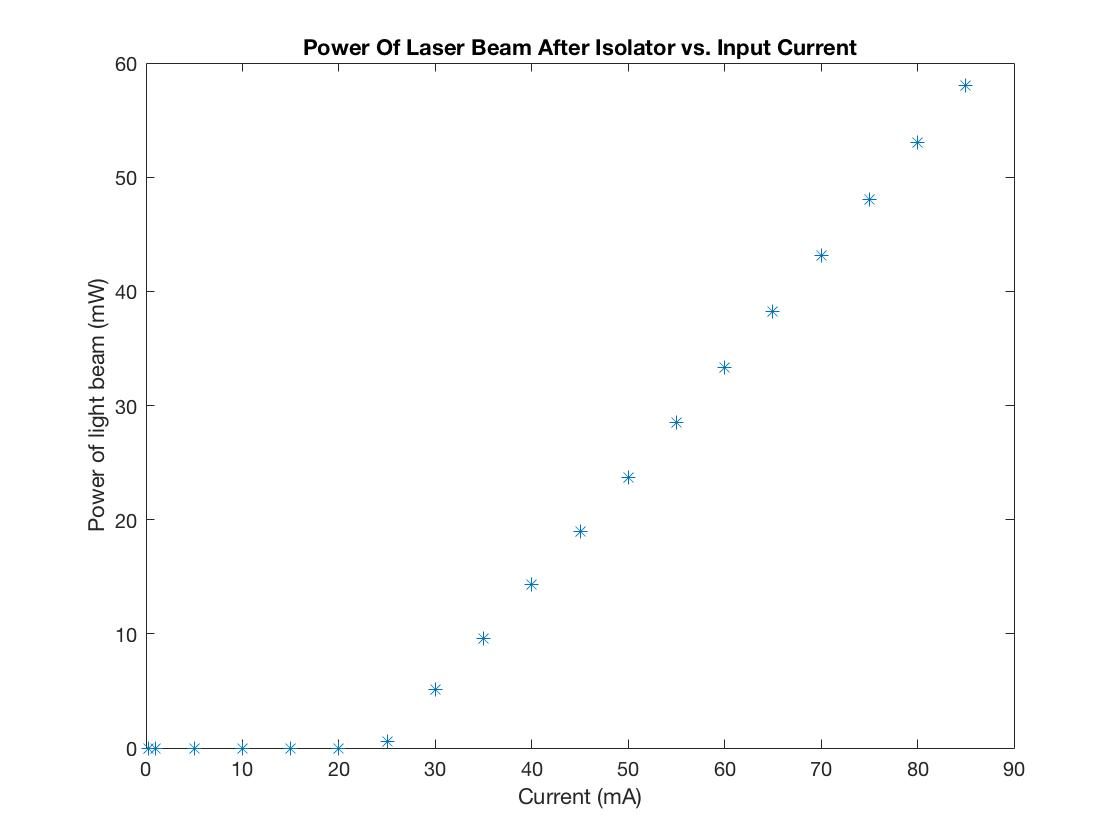
\includegraphics[scale = 0.15]{1.jpg}
    \caption{}
    \label{fig:my_label}
\end{figure}

   FINISH,    